%% Copernicus Publications Manuscript Preparation Template for LaTeX Submissions
%% ---------------------------------
%% This template should be used for copernicus.cls
%% The class file and some style files are bundled in the Copernicus Latex Package, which can be downloaded from the different journal webpages.
%% For further assistance please contact Copernicus Publications at: production@copernicus.org
%% https://publications.copernicus.org/for_authors/manuscript_preparation.html


%% Please use the following documentclass and journal abbreviations for preprints and final revised papers.

%% 2-column papers and preprints

\documentclass[amt, manuscript]{copernicus}
%\documentclass[amt]{copernicus}

%\documentclass[amt]{copernicus}




%% Journal abbreviations (please use the same for preprints and final revised papers)

%% \usepackage commands included in the copernicus.cls:
%\usepackage[german, english]{babel}
%\usepackage{tabularx}
%\usepackage{cancel}
%\usepackage{multirow}
%\usepackage{supertabular}
%\usepackage{algorithmic}
%\usepackage{algorithm}
%\usepackage{amsthm}
%\usepackage{float}
%\usepackage{subfig}
%\usepackage{rotating}

\newcommand{\todo}[1]{{\color{red} #1}}

\begin{document}

\title{Cloud correction and filtering of operational microwave humidity
  radiances with case specific uncertainty estimation}


\Author[1]{Inderpreet}{Kaur}
\Author[1]{Patrick}{Eriksson}
\Author[1]{Simon}{Pfreundschuh}

\affil[1]{Department of Space, Earth and Environment, Chalmers University of
  Technology, Gothenburg, Sweden} 

%% If authors contributed equally, please mark the respective author names with an asterisk, e.g. "\Author[2,*]{Anton}{Aman}" and "\Author[3,*]{Bradley}{Bman}" and add a further affiliation: "\affil[*]{These authors contributed equally to this work.}".


\correspondence{Inderpreet Kaur <kauri@chalmers.se>}

\runningtitle{Cloud correction with case specific uncertainty estimation}

\runningauthor{Kaur et al.}

\firstpage{1}

\maketitle


\begin{abstract}
TEXT
\end{abstract}


\copyrightstatement{TEXT}


\introduction
%
Satellite observations of humidity inside the troposphere are mainly performed
by downward-looking sensors. Among this class of observations, the frequency
range around 183\,GHz has a special position. Water vapour has a noticeable
transition at 22\,GHz, but it is relatively weak and only column values can be
derived \citep[e.g.][]{schluessel1990atmospheric} for the observation geometry
of concern. The first transition in the microwave region that can be used to
derive altitude information, i.e.\ can be used for ``sounding'', is the one at
183.31\,GHz \citep{kakar1983retrieval,wang1983profiling}. On the other hand, at
infrared wavelengths a high number of water vapour transitions are found,
including some of high strength. As a consequence, infrared sounders can
provide humidity profiles with high precision and good vertical resolution, but
with strong limitations imposed by clouds. To be able to also sense humidity
inside and below clouds weather satellites are since some time equipped with
channels around 183\,GHz. Today such channels are part of several sensors, such
as ATMS (Advanced Technology Microwave Sounder, \citet{weng2012introduction}).

Precipitation and most dense clouds, particularly if found at high altitude, can
still affect measured radiances around 183\,GHz
\citep[e.g.][]{bennartz2003sensitivity}. As the impact from the hydrometeors
then is dominated by scattering, the complexity of the analysis of the data
increases dramatically and there exists a need to identify the problematic
cases. This is normally denoted as cloud filtering, to obtain data of ``clear
sky'' character. Such filtering has been applied to derive climate records
\citep{lang2020new} and is essential in studies of the agreement between
observations and simulations \citep{brogniez2016review} as well as 
comparing observations of different instruments to validate their calibration
\citep{john2013assessment,moradi:retri:15,berg2016intercalibration}. A commonly
used cloud filtering methods for these applications is the one of
\citet{buehler:aclou:07}. This method is based on the 183\,GHz data alone,
involving rules on the brightness temperatures differences between channels. An
older version is \citet{burns1997effects}.

The main motivation for introducing 183\,GHz channels in operational sensors is
numerical weather prediction (NWP). Usage of microwave data by ``all-sky''
assimilation is growing \citep{geer2017growing}, but 183\,GHz data are still
mainly used in a clear sky fashion \citep{geer2018all}. The later is
particularly true in NWP of regional scope, all-sky assimilation of 183\,GHz at
many national weather agencies will likely not be reached in many years. The
cloud filtering in NWP differs between centres. One approach is to make use of
a ``scattering index'' \citep{bennartz2002precipitation}, based on the
observations alone. Today, likely more common is to use ``observation minus
background'' (O-B), where the forecast model is used to obtain an estimate of
the expected clear-sky value and the observation is rejected if the deviation
exceeds some threshold (???). In both cases, the filtering typically involves
observations around 89 and/or 150\,GHz.

Despite the broad usage these filtering methods have some drawbacks. For
183\,GHz, the impact of hydrometeors systematically causes a decrease in the
observed radiance (maybe with exceptions at extremely dry conditions), see
e.g.\ \citet{barlakas:three:20} and below. This means that if any cloud
contamination is missed by the filtering this will cause a negative bias in
mean radiance, compared to the true clear-sky mean. This bias will translate to
a bias in humidity after the retrieval or assimilation. The alternative is to
apply a very strict filtering, but this will result in that a high fraction of
actually clear-sky values will be rejected \todo{(Reka or better reference)},
i.e.\ an important loss of useful data.

The filtering is normally done in a ``one for all'' manner, i.e.\ all 183\,GHz
channels are either kept or rejected, while, as the channels differ in their
altitude coverage, there could be cloud impact in some channels and still the
others can be considered as clear-sky. To allow a channel specific filtering,
data likely need to be combined in a more complex manner than simple
differences, but it is unclear what type of regression that would be best. This
points towards applying machine learning, as used by e.g.\
\citet{favrichon2019detecting}.

A maybe less obvious problem is the uncertainty to assign to the filtered
values. To our best knowledge, in best case estimates of mean and worst case
errors are provided. Some cases with relatively high cloud impact will likely be
missed, while most cases are clear sky from start. As the remaining cloudy
cases can cause significant biases, the likely solution is to apply a quite
conservative (high) error estimate. However, this will unnecessary downgrade
the value of the truly clear sky cases and the observations are used in a
non-optimal manner.

We are here approaching cloud filtering task from a new angle. The basic idea
is to derive an estimate of the corresponding noise-free clear-sky (NFCS) value
(i.e.\ the radiance that would have been measured in absence of noise and
hydrometeors). This is done for each channel separately, only using
measurements (no ``background'' data involved). Not only a best estimate is
provided, but also a case specific uncertainty.

This information can be used as a pure filter, by rejecting data where the
correction exceeds some threshold value. This threshold value should be
relatively low, to not introduce a bias in filtered dataset. However, even
better is to replace the original value with the predicted NFSC value when
forming the clear-sky dataset. This approach we denote as cloud correction. It
is shown below that a basically bias free cloud correction can be obtained.
This feature removes the need of threshold value, as long as the retrieval or
assimilation system can incorporate the uncertainty of the corrected value. As
also will be shown, the uncertainty for originally clear sky data is determined
by noise, but the uncertainty increases with magnitude of correction.
Accordingly, the cloud correction approach allows that the full weight of
clear-sky data can be preserved.

The estimation of NFSC values makes use of a special type of machine learning,
denoted as Quantile Regression Neural Network (QRNN,
\citet{pfreundschuh:aneur:18}). Unlike standard usage of machine learning where
only some kind of best estimate is provided, QRNN works in a Bayesian fashion
and instead gives a description of the posterior uncertainty. More precisely,
QRNN outputs an user specified set of percentiles that gives a discrete
description posterior distribution, that can be process to derive e.g.\ the
expectation value.

The approach is demonstrated on a combination of 183\,GHz channels (following
\citet{buehler:aclou:07}), but we mainly explore the cloud correction (of
183\,GHz data) that will be possible when sub-millimetre data will be at hand
in some years. This wavelength region will be introduced by the Ice Cloud
Imager (ICI, \citet{eriksson:towar:20}), but likely also be included in several
smaller missions (such as AWS presented below). The focus on ICI is motivated
by several reasons. The true potentail of the QRNN cloud correction approach is
likely not revealed if tested on existing data and applying ICI data for cloud
filtering has not earlier been discussed. It is also argued that the cloud
correction makes it possible to make good use of ICI data already in clear-sky
assimilation, a fact that should speed up the use of this novel data source.



\newpage

\section*{Outline of sectioning}

2 Data and methods

2.1 Satellite sensors

2.1.1 Ice Cloud Imager (ICI)

2.1.2 Microwave Imager (MWI)

2.1.3 Arctic Weather Satellite (AWS)

2.2 Quantile Regression Neural Network (QRNN)

2.2.1 Theory

2.2.2 Evaluation metrics

2.3 Simulations

2.3.1 Input data

2.3.2 Simulation setup

2.3.3 Produced dataset
(If diifers between ICI, MWI and AWS, clarify this)

\noindent 3 Results

Short recap of aim of correction. We also use the correction as a filter, using
a threshold on the correction. We use 5K (?) threshold as example.

3.1 QRNN network configurations and training

3.2 ICI

3.2.1 Example results

Show a few estimated posterior distributions (one figure) and distribution of
predicted values (Fig 2)

3.2.2 Error of best estimate

3.2.3 Predicted uncertainty

3.3 MWI

3.3.1 MWI alone

Just 183 GHz channels, original noise

3.3.2 MWI and ICI

As in present version

3.4 AWS

\noindent 4 Discussion

\noindent 5 Conclusion


\newpage
\section{Data and methods}



\subsection{Ice Cloud Imager}
%
%t
\begin{table*}[t]	
	\caption{Specifications of ICI and MWI channels. For MWI only 183\,GHz channels are shown.}
	\label{tab:ICI_MWI_channels}
	\begin{tabular}{lrrrr}
		\tophline
		Channel & Frequency 	& Bandwidth  	&NE$\Delta$T	&Polarisation\\
				& [GHz]			& [MHz]			& [K]			&\\
		\middlehline
		I1V&	183.31$\pm$7.00    & 2000 			& 0.8 		& V\\
		I2V&	183.31$\pm$3.40    & 1500 			& 0.8 		& V\\
		I3V&	183.31$\pm$2.00    & 1500			& 0.8 		& V\\
		I4V&	243.20$\pm$2.50    & 3000			& 0.7 		& V\\
		I4H&	243.20$\pm$2.50    & 3000			& 0.7 		& H\\
		I5V&	325.15$\pm$9.50    & 3000			& 1.2 		& V\\
		I6V&	325.15$\pm$3.50    & 2400			& 1.3 		& V\\
		I6V&	325.15$\pm$1.50    & 1600			& 1.5 		& V\\
		I8V&	448.00$\pm$7.20    & 3000			& 1.4 		& V\\
		I9V&	448.00$\pm$3.00    & 2000			& 1.6 		& V\\
		I10V&	448.00$\pm$1.40    & 1200			& 2.0 		& V\\
		I11V&	664.00$\pm$4.20    & \phantom{0}500			& 1.6 		& V\\
		I11H&	664.00$\pm$4.20    & \phantom{0}500 			& 1.6 		& H\\		
		\bottomhline
	\end{tabular}
	\begin{tabular}{lrrrr}
		\tophline
		Channel & Frequency 	& Bandwidth  	&NE$\Delta$T	&Polarisation\\
				& [GHz]			& [MHz]			& [K]			&\\
		\middlehline
		MWI-14&	183.31$\pm$7.00    & 2000 			& 1.3 		& V\\
		MWI-15&	183.31$\pm$6.10    & 1500			& 1.2 		& V\\
		MWI-16&	183.31$\pm$4.90    & 1500			& 1.2 		& V\\
		MWI-17&	183.31$\pm$3.40    & 1500			& 1.2 		& V\\
		MWI-18&	183.31$\pm$2.00    & 1500			& 1.3 		& V\\	
		\bottomhline
	\end{tabular}

	\belowtable{} % Table Footnotes
\end{table*}

Ice Cloud Imager (ICI) is a new EPS-SG (EUMETSAT Polar System - Second Generation) sensor that will observe  Earth using submillimeter-wave (sub-mm) frequency range. The main objective of ICI is measure ice cloud properties and improve the representation of clouds in regional and global models. ICI is a conically scanning millimetre/sub-millimetre radiometer which will measure 13 frequencies from 183 GHz up to 664 GHz. Channels with centre frequencies 183.31, 325.15 and 448.0\,GHz are centered on water vapor absorption lines, and measure vertical polarization. While other channels around 243.0 and 664.0\,GHz are ``window channels'' and receive both vertical and horizontal polarization. 

\subsection{MicroWave Imager}
%
In addition to ICI, the EPS-SG satellite will also have Microwave Imager (MWI) onboard. MWI will measure frequencies from 18.7 GHz up to 183\,GHz and provide data continuity to the existing microwave imager measurements. The common 183\,GHz channels among the two instruments shall allow cross-calibration between the two instruments. A brief summary of the MWI 183\,GHz channels is provided in Table~\ref{tab:ICI_MWI_channels}.

\subsection{Artic Weather Satellite}
%
\begin{table*}[t]
	\caption{Specifications of AWS channels around 183\,GHz and 325\,GHz.}
	\label{tab:specifications_AWS}	
	\begin{tabular}{lrr}
		\tophline
		Channel & Frequency 	& Bandwidth  \\
		& [GHz]			& [MHz]		\\
		\middlehline
		AWS-32	&	176.311    & 2000 		\\
		AWS-33	&	178.811    & 2000 		\\
		AWS-34	&	180.311    & 1000 		\\
		AWS-35	&	181.511    & 1000 		 \\
		AWS-36	&	182.311    & \phantom{0}500 	 \\
		AWS-41    & 325.15$\pm$6.60    & 2800 \\
		AWS-42    & 325.15$\pm$4.10    & 1800  \\
		AWS-43    & 325.15$\pm$2.40    & 1200 \\
		AWS-44    & 325.15$\pm$1.20    & \phantom{0}800  \\
		\bottomhline
	\end{tabular}
	\belowtable{} % Table Footnotes
\end{table*}

The Arctic Weather Satellite (AWS) is a small satellite mission approved as ESA
Earth Watch Programme Element. It is a small platform carrying a single
across-track scanning microwave radiometer. It is planned as a small but cost-effective platform, which can supplement the information from other polar orbiting satellites. The main objective of AWS will be to improve representation of Artic and sub-Arctic weather in NWP models and improve the global weather forecasts. AWS will will have channels receiving frequencies around 89\,GHz, 165.5\,GHz, 183\,GHz, 229\,GHz and 325\,GHz. For a detailed description of the AWS channels see \citet{eriksson2020study}, while a brief summary of AWS channels relevant to this study are provided in
Table~\ref{tab:specifications_AWS}. The first prototype mission is expected to be delivered around 2023. 

\subsection{QRNN}
%
The neural network training is a process of learning to predict the outputs {$y_i$} from inputs {$x_i$} through a series of learnable transformations. While training, neural networks seek to minimise the model error through a loss function. The choice of the loss function depends on the predictive problem. When a neural network is trained to minimise the mean of the quantile loss function to predict the quantiles of the distribution, it is called a Quantile Regression Neural Network (QRNN). 
\subsubsection{Theory}

\subsubsection{Evaluation metrics}

Quantile loss function

CRPS

\subsection{Simulations}
\label{sec:arts_simulations}
%
\subsubsection{Input data}
%
\subsubsection{Simulation setup}
%
**** Some parts copied directly from AWS report *****

The satellite observations for all ICI channels are simulated with the Atmospheric Radiative Transfer Simulator (ARTS, (ARTS, \citet{eriksson:arts2:11,buehler:artst:18})version. The simulations include TB from five ICI channels around 183\,GHz, 243\,GHz, 325\,GHz, 448\,GHz and 664\,GHz. 

The absorption model takes into account the effect from nitrogen
\citep{pwr:93}, oxygen \citep{pwr:93} and water vapour
\citep{ellison2007permittivity}. LWC is taken from ERA-Interim and is assumed
to be totally absorbing. In the mapping of CloudSat reflectivities to RWC and
IWC a total separation between liquid and ice phase is assumed. All scattering
hydrometeors at temperatures above 0$^\circ$C are assumed to be rain, and all
below 0$^\circ$C are assumed to be ice hydrometeors. For RWC the particle size
distribution of \citet{abel2012improved} is applied. The PSD of IWC follows the
basic formulation applied in DARDAR (\verb
 http://www.icare.univ-lille1.fr/projects/dardar), using latest parameter
 values (i.e.\ $\alpha$ and $\beta$) as given by \citet{cazenave2019evolution}.
 This PSD can be considered as a ``two moment'' scheme, but is here applied in
 a one moment manner by setting $N_0^*$ (as a function of temperature)
 following Table~5 of \citet{delanoe2014normalized}, and letting the radar
 reflectivity set the remaining moment. Single scattering data are taken from
 \citet{eriksson:agene:18}. For ice hydrometeors, three habits are applied:
 Perpendicular 3-bullet rosette, Large plate aggregate and Large column
 aggregate. In the last two cases, the aggregates are complemented with single
 crystal data to also cover smaller sizes. These data describe particles
 assumed to have a totally random orientation. To apply oriented particles is
 much more computationally costly and could not be accommodated inside the
 study. The land emissivity was taken from TELSEM \citep{aires2011tool} and the
 Ocean/water from TESSEM \citep{prigent2017sea}. For each atmopsheric case,
 both ''clear-sky'' and ``all-sky'' calculations were performed. In the former,
 all impact of all hydrometeors were set to zero, while in the latter, IWC and
 RWC derived from CloudSat reflectivities and LWC from ERA-Interim were taken
 into account. Both sets of calculations were made by ARTS's interface to the
 RT4 solver \citep{evans1995microwavec}. To avoid a possible bias between
 clear-sky and all-sky for insignificant hydrometeor contents, the same
 ``scattering solver'' was used for both calculations. The first two elements
 of the Stokes vector were calculated.

\subsection{Produced dataset}
%
Using the simulation setup described in previous section, Cloudsat profiles during August 2015 were randomly selected to generate 220\,000 cases for each ICI and MWI frequency. The input data were restricted between $60^{\degree}$S to $60^{\degree}$N, and surface is below 500\,m. Both clear-sky and all-sky scenarios were simulated, and no differentiation was made between the observations over ocean/sea and land. It is also assumed that all simulations of ICI and MWI are remapped to a common foorprint. 

For AWS, 7 monochromatic frequencies were simulated each for 183\,GHz, 325\,GHz-upper amd 325\,GHz-lower, so that the channel brightness temperature for each could be represented with sufficient accuracy. The monochromatic frequencies were interpolated to a finer grid to get the channel temperatures. All AWS sensor viewing angles (from $0^\circ$ to $45^\circ$) were simulated, but the results described in this section are based on nadir viewing angle. 130\,000 cases based on randomly selected CloudSat orbits were simulated.

\begin{table*}[t]
	\caption{Summary of the different QRNN models used in the study.}
	\label{tab:QRNN_models}
	\begin{tabular}{lllll}
		\tophline
		QRNN model & Sensor & Target & Input 183\,GHz channel(s) &Other training inputs \\
		\middlehline
		QRNN-single &  ICI 	& I1V/I2V/I3V 	& I1V/I2V/I3V, & I5V, I6V, I7V, I8V, I9V, I10V, I11V\\
		\cline{2-5}
					&  MWI 	& MWI-15/MWI-16 & MWI-15/MWI-16	& I5V, I6V, I7V, I8V, I9V, I10V, I11V \\
		\cline{2-5}
					& AWS	& AWS-32/AWS-33/ &  AWS-32/AWS-33/ & AWS-41, AWS-42, AWS-43, AWS-44\\
					&		& AWS-34/		 &	AWS-34/		   & \\
					&		& AWS-35/AWS-36	 & AWS-35/AWS-36,  &\\
		\cline{1-5}
		QRNN-all &  ICI 	& I1V/I2V/I3V 	& I1V, I2V, I3V & I5V, I6V, I7V, I8V, I9V, I10V, I11V\\
		\cline{1-5}
		QRNN-mwi &  MWI		& MWI-14/MWI-15/ &  MWI-14, MWI-15, & None 	\\	
				 &			& MWI-16/		 &  MWI-16, & \\
				 &			& MWI-17/MWI-18	 &  MWI-17, MWI-18  &\\					
	\bottomhline
\end{tabular}
\belowtable{} % Table Footnotes
\end{table*}						


\subsection{Training data}
%
The QRNN models presented in this study are trained with simulated brightness temperature data to predict the NFSC values for 183\,GHz channels. No other data was included in the training process, but the training set varied according to the QRNN-model (described further). Out of the 220\,000 simulations for ICI and MWI each, 175\,000 cases were randomly picked to form the training set. The rest were used for testing. For AWS a slightly smaller database was selected. We had 130\,000 available simulations and all were used for training. A testing dataset was constructed by randomly drawing 25\,000 cases from the training dataset and noise was added to each simulation to mimic a new measurement set. 

In the training set for all three sensors, 90\% of the data was randomly selected to form the training set, while the other 10\% formed the \textit{testing-during-training} database. ARTS simulations are noise free, so to incorporate the satellite measurement uncertainties, gaussian noise was added to the input training data according to the channel NE$\Delta$T. The target training data was kept noise free. In order to build a robust learning network, random noise was added to the inputs at each training iteration. This exposes the model to a different datasets during the entire training process and avoids the memorisation of training samples. The input data was also normalized with mean and standard deviation.  

\subsection{QRNN model configurations}
%
\label{QRNN_models}
Multiple QRNN models were trained with several combinations of the training input. For each combination, the target was always one of the available 183\,GHz channels, and this target channel was always included in the training set. The choice of other channels in the training set depended on the type of QRNN model chosen. Three main types of QRNN models were used in this study. 

In the first model, the training inputs always contained data from the target 183\,GHz channel, and one or more available sub-mm channels. No data from other 183\,GHz channels was included in training. We refer this model as ``QRNN-single''. For ICI and MWI, the available sub-mm channels are 325\,GHz, 448\,GHz and 664\,GHz, while for AWS only 325\,GHz is available. It should be noted that though MWI does not have any sub-mm channels,  sub-mm channels from ICI were used. It is assumed for the simulations that data from ICI and MWI channels are mapped to a common footprint and resolution. In such case, remapping reduces the noise in MWI channels from 1.2\,K at 10\,Km resolution to 0.8\,K at 15\,Km resolution. 
 
The second model was defined to investigate the  impact of using all 183\,GHz channels concurrently. This model is referred as ``QRNN-all''. In this model, the training set included data from all available 183\,GHz channels, along with other sub-mm channels. This model was applied only to ICI. It should be noted that although the training set was identical for I1V, I2V and I3V, a separate training was needed for each channel as target.

The third model was used only for MWI channels. In this case, all 183\,GHz channels were used concurrently in the training set. No other data from sub-mm channels was used. Further in the text, we shall refer this model as ``QRNN-mwi''. 

A summary of the three QRNN models described in this study is provided in Table~\ref{tab:QRNN_models}.

\section{Results}
%
In this section, QRNN is used to predict the NFCS values for operational humidity channels. The main aim of this study is to demonstrate that sub-mm channels can be used to formulate the cloud filtering/correction of data measured around 183\,GHz. Different combinations of 183\,GHz channel and sub-mm channels are applied to QRNN and the results are compared. To determine the prediction performance of QRNN, the NFCS simulations are used as reference. Results from both pure-filtering and correction are described. Furthermore, the case specific uncertainties obtained from QRNN are also discussed.
 
\subsection{QRNN network structure}
%
A high performing QRNN model requires tuning of multiple hyper-parameters. These parameters determine the structure and the training set-up of the neural network. Several of these hyper-parameters are non-learnable, and must be defined before beginning of every training. Grid search is one of the most often employed techniques for hyper-parameter tuning. In grid search, different combinations of hyper-parameters are selected and for each, the model performance is evaluated. The model architecture with the best performance is selected. We use quantile loss and CRPS for evaluation of the model performance. 

For the structural parameters, usually a grid search over the number of neurons (width) and hidden layers (depth) is performed. The model is trained for multiple values of layer widths and hidden layers, and the best configuration is selected by evaluating the predictions over validation dataset. Similarly, the training process is optimized by performing a grid search different training parameters such as : batch size, learning rate, number of epochs etc. In this study, all possible hyper-parameters were not tested. We investigated the performance of QRNN only to certain hyper-parameters like number of neurons, hidden layers, learning rate, convergence epochs and batch size. The others were chosen empirically.

Firstly, we performed a grid search to select the size of the neural network. We evaluated the performance for three sizes of hiddden layers($n_h$ = 2, 3, 4), and layer widths of sizes in the set [8, 16, 32, 64, 128, 256, 512]. The mean quantile loss and CRPS for different layer width and hidden layer configurations are shown in Fig\ref{fig:grid_search}. The results are for QRNN-single with I2V as target channel. Increasing the complexity of the network by increasing the layer width and depth has a positive impact on performance. However for four hidden layers, increasing the number of neurons beyond 128 has no significant impact on the performance. On basis of these results, a neural network with four hidden layers and 128 neurons in each layer was selected for QRNN-single. For the optimising the training parameters, a customised  learning rate scheduler was implemented. The initial learning rate was reset after a certain number of epochs.  We started the training process with a initial learning rate of 0.1, and decreased it by a factor of 10 after 100 epochs. The best neural network performance was obtained when the network was trained three times with a new initial learning rate. For each training  if the validation loss remained unchanged till 6 training epochs, the learning rate was reduced by a factor of 2. In order to select the batch size, we simply compared the performance for batch size = 128 and 256, and the former gave better results. Concerning number of maximum epochs, we obtained best results when the network was trained longer. Choosing a lower value of epochs (e.g. 50), did not affect the accuracy of the median value, yet deteriorated the prediction uncertainty. We did not optimise the type of activation function and Rectified Linear Unit (ReLu) was used in all layers. 

Though these set of hyper-parameters were selected for QRNN-single applied to I2V, they worked well for other channnels and QRNN-all/QRNN-mwi as well. In the end, all the results described in this study use an identical hyper-parameter configuration.

\begin{figure*}[t]
	\centering
	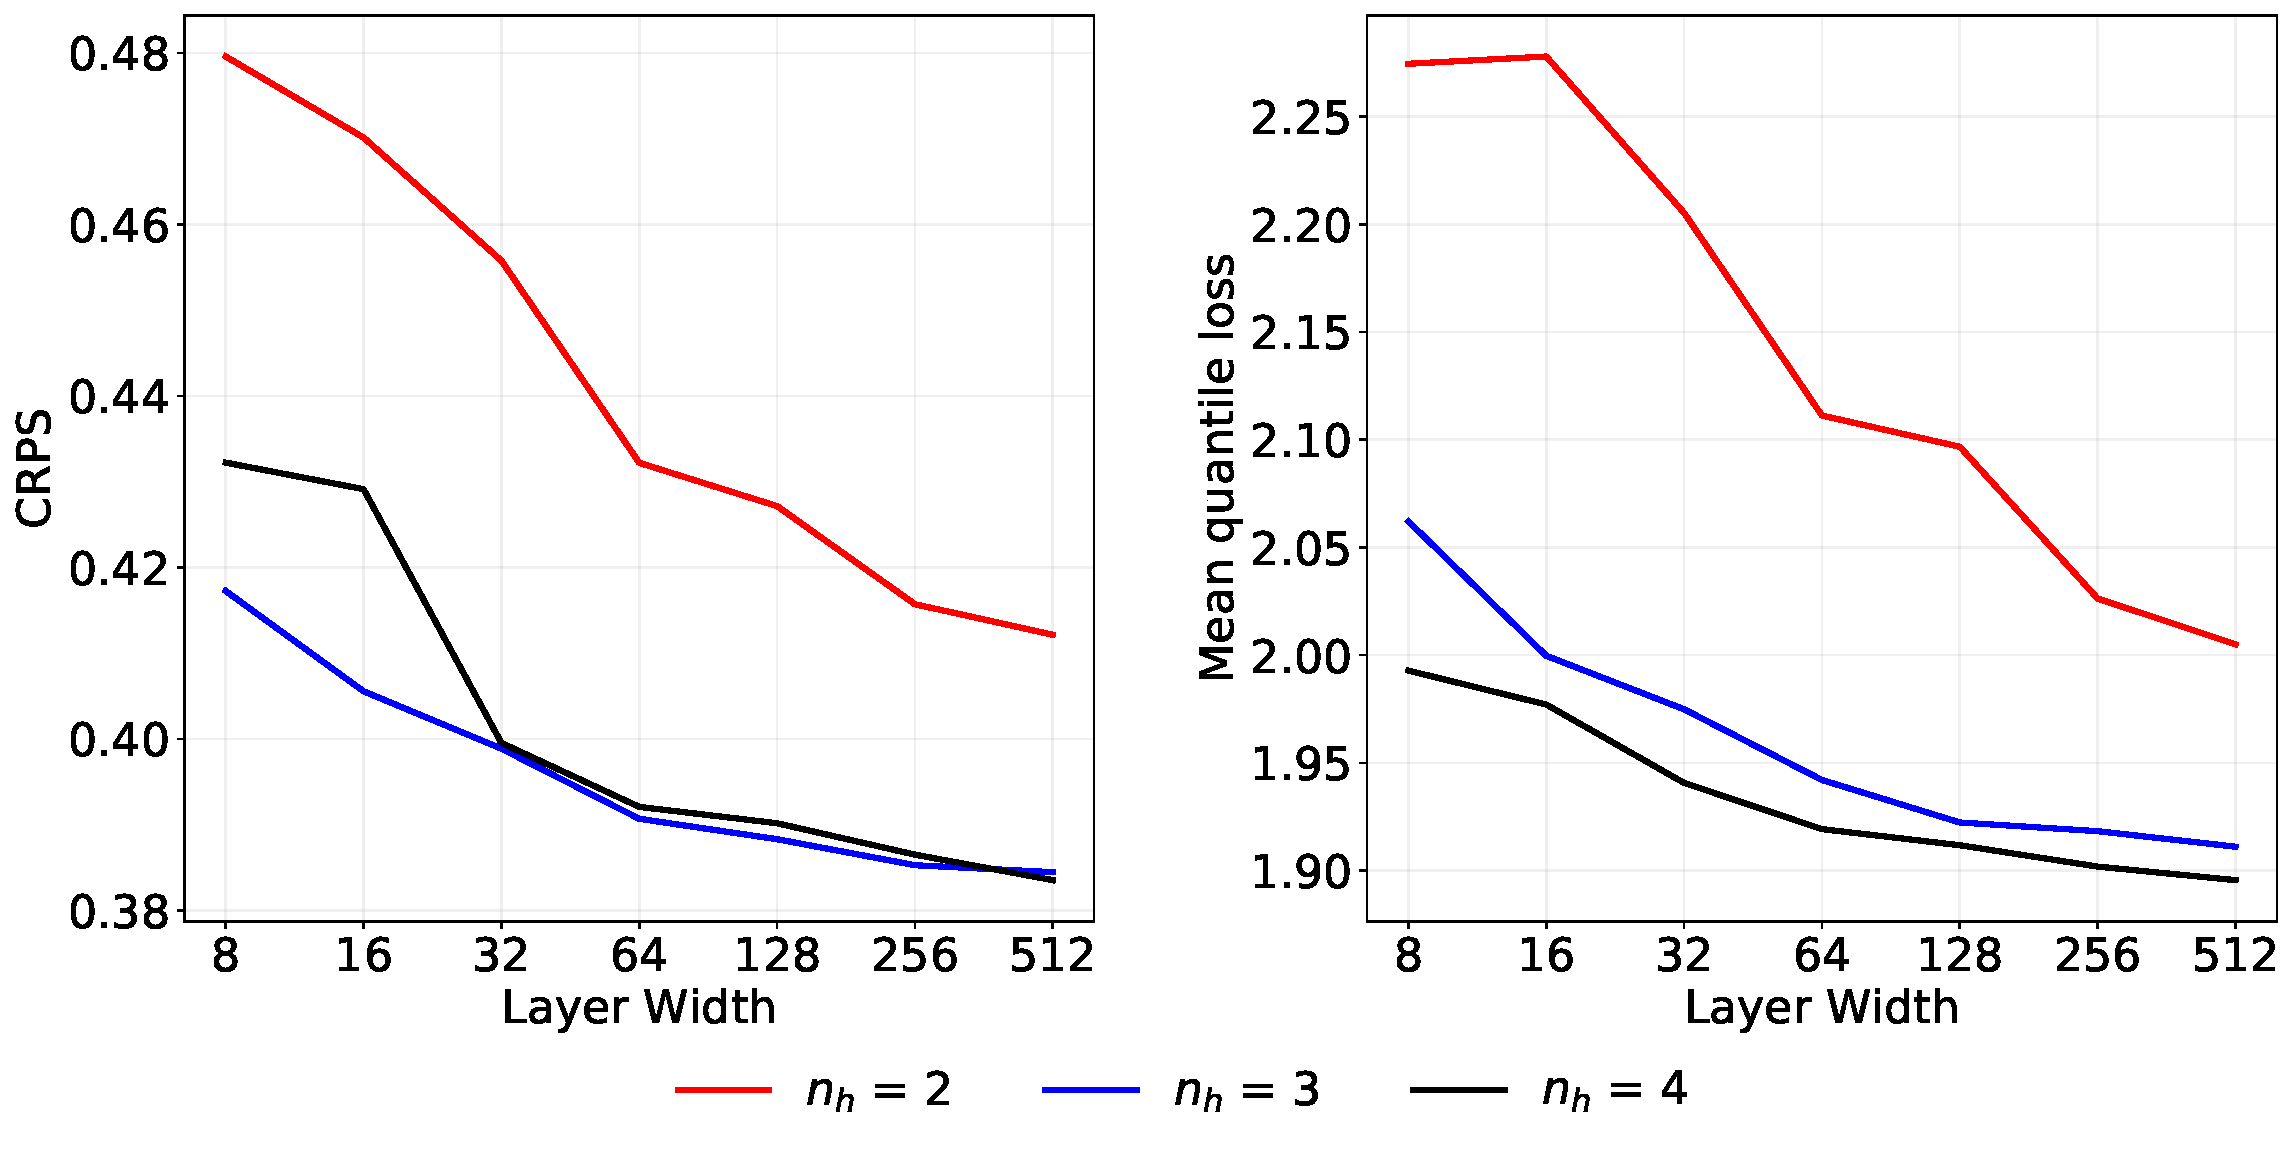
\includegraphics[height=60mm]{Figures/CRPS.pdf} 
	\caption{CRPS(left) and mean quantile loss(right) for different combinations of layer width and hidden layers ($n_h$). The results are from QRNN-simple for channel I2V.}
	\label{fig:grid_search}	
\end{figure*}


\subsection{ICI}
\subsubsection{Example results}
%
QRNN predictions are estimates of the posterior distribution over different quantiles. For this study we chose quantiles, $x_{\tau}$: median, $\pm 1\sigma$, $\pm 2 \sigma$ and  $\pm 3 \sigma$ ($\tau$ = 0.002, 0.03, 0.16, 0.5, 0.84, 0.97, 0.998). The quantiles are interpreted as probabilistic predictions and can be used to construct a probability distribution of the predictions. This is in sharp contrast to correction approaches which give out only point estimates. As an example, Fig.~\ref{fig:posterior_distribution_I2V} shows the posterior distribution obtained from QRNN for three different cases. These results are from QRNN-single for channel I2V. The three cases shown in the figure have almost a similar median value but very different spread. The spread of the distributions can also be expressed as the prediction interval. If $y_{\tau_2}, y_{\tau_1}$ are the predictions at two quantile levels $\tau_1$ and $\tau_2$ respectively, the interval $[y_{\tau_2}, y_{\tau_1}]$ is called the prediction interval. It is gives the range where the prediction could be located and its length is a measure of the reliability. Among the three cases shown in the figure, the blue curve has shortest prediction interval indicating a sharp probabilistic prediction or more reliability. While the other two cases have longer intervals implying higher fluctuations, or low reliability.

The quantiles can also be used to  interpret the confidence intervals. For a given case, if two quantiles $\tau_1$ and $\tau_2$ are chosen, then there is $\tau_2 - \tau_1$ chance that the true value ($y_o$) shall lie in in range $[y_{\tau_1}, y_{\tau_2}]$. For example, in a 94\% confidence interval where, $\tau_1 = -2\sigma$ and $\tau_1 = +2\sigma$, there is 0.3\% probability that $y_\circ > y_{\tau_2}$, and 97\% probability that $y_\circ$ > $y_{\tau_1}$. 

%f
\begin{figure}[t]
	\centering
	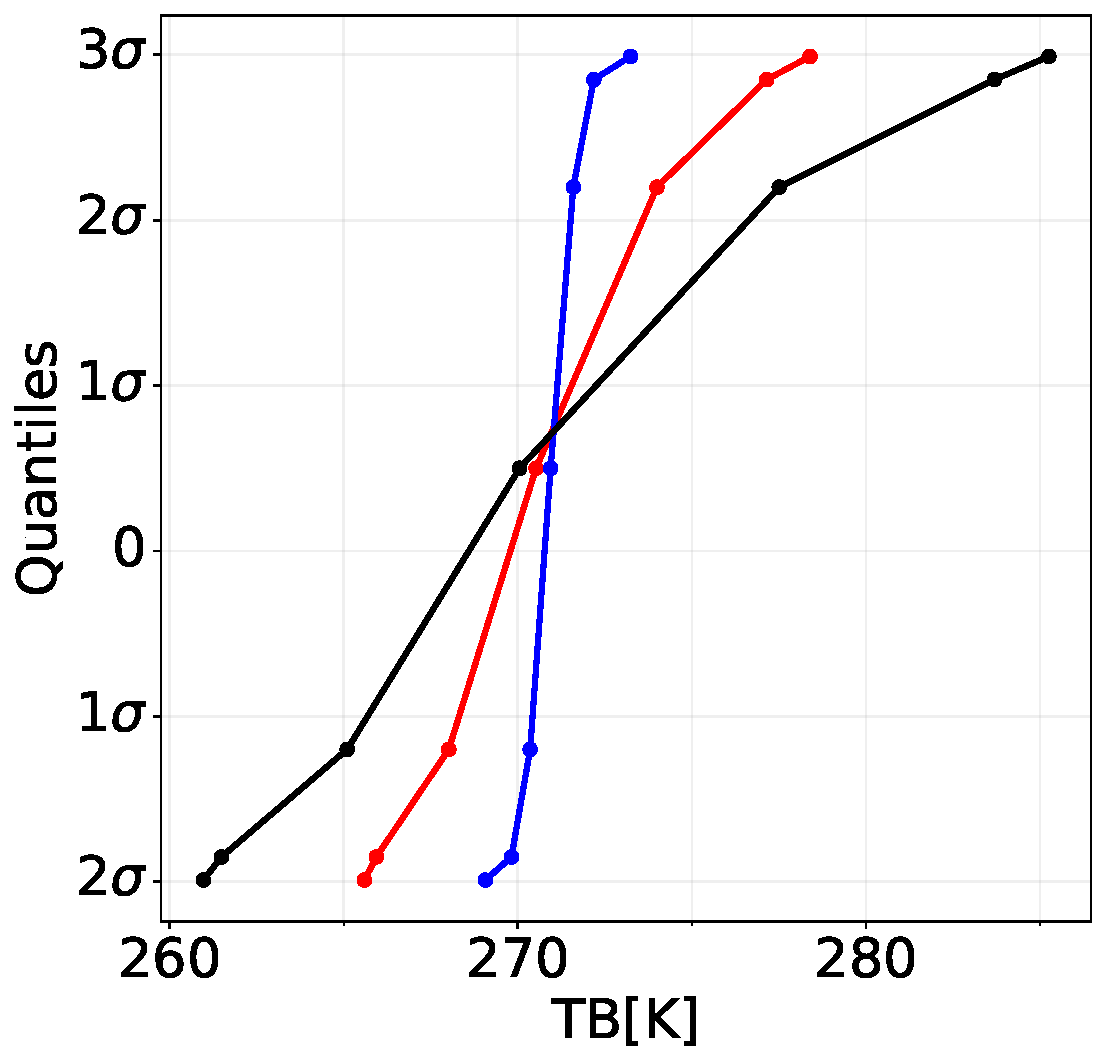
\includegraphics[height=60mm]{Figures/posterior_distribution_I2V.pdf} 
	\caption{Posterior distribution obtained from QRNN-single (channel I2V) for three different cases. }
	\label{fig:posterior_distribution_I2V}	
\end{figure}

\subsubsection{Error of best estimate}
%
%f
\begin{figure*}[t]
	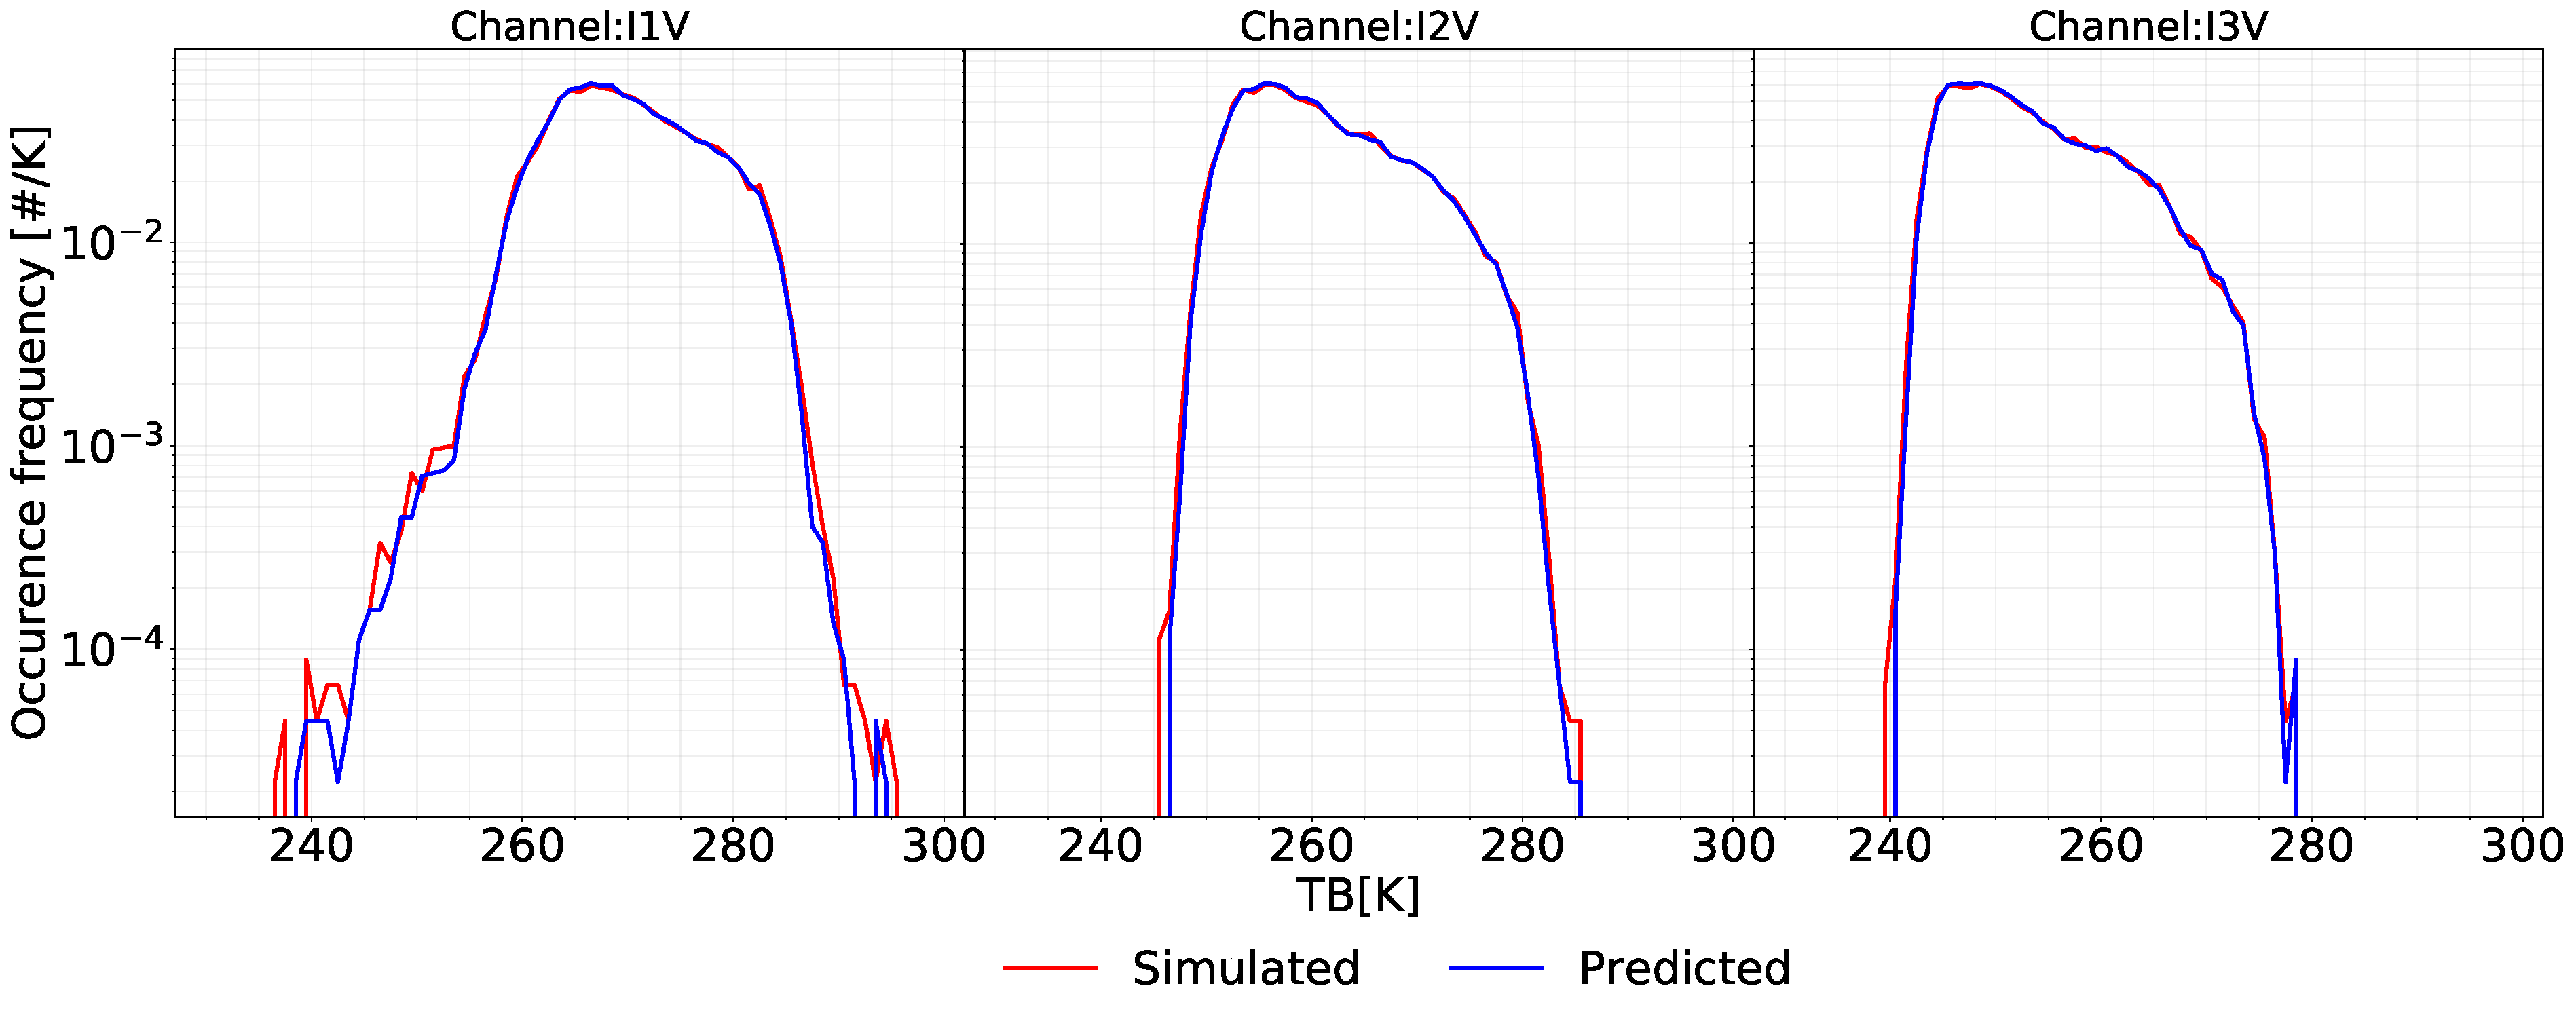
\includegraphics[width=\textwidth]{Figures/PDF_predictions_ICI.pdf} 
	\caption{Distributions of predicted clear-sky values from QRNN-simple for channels I1V, I2V and I3V. }
	\label{fig:PDF_predictions}	
\end{figure*}
%f 
\begin{figure*}[t ]
	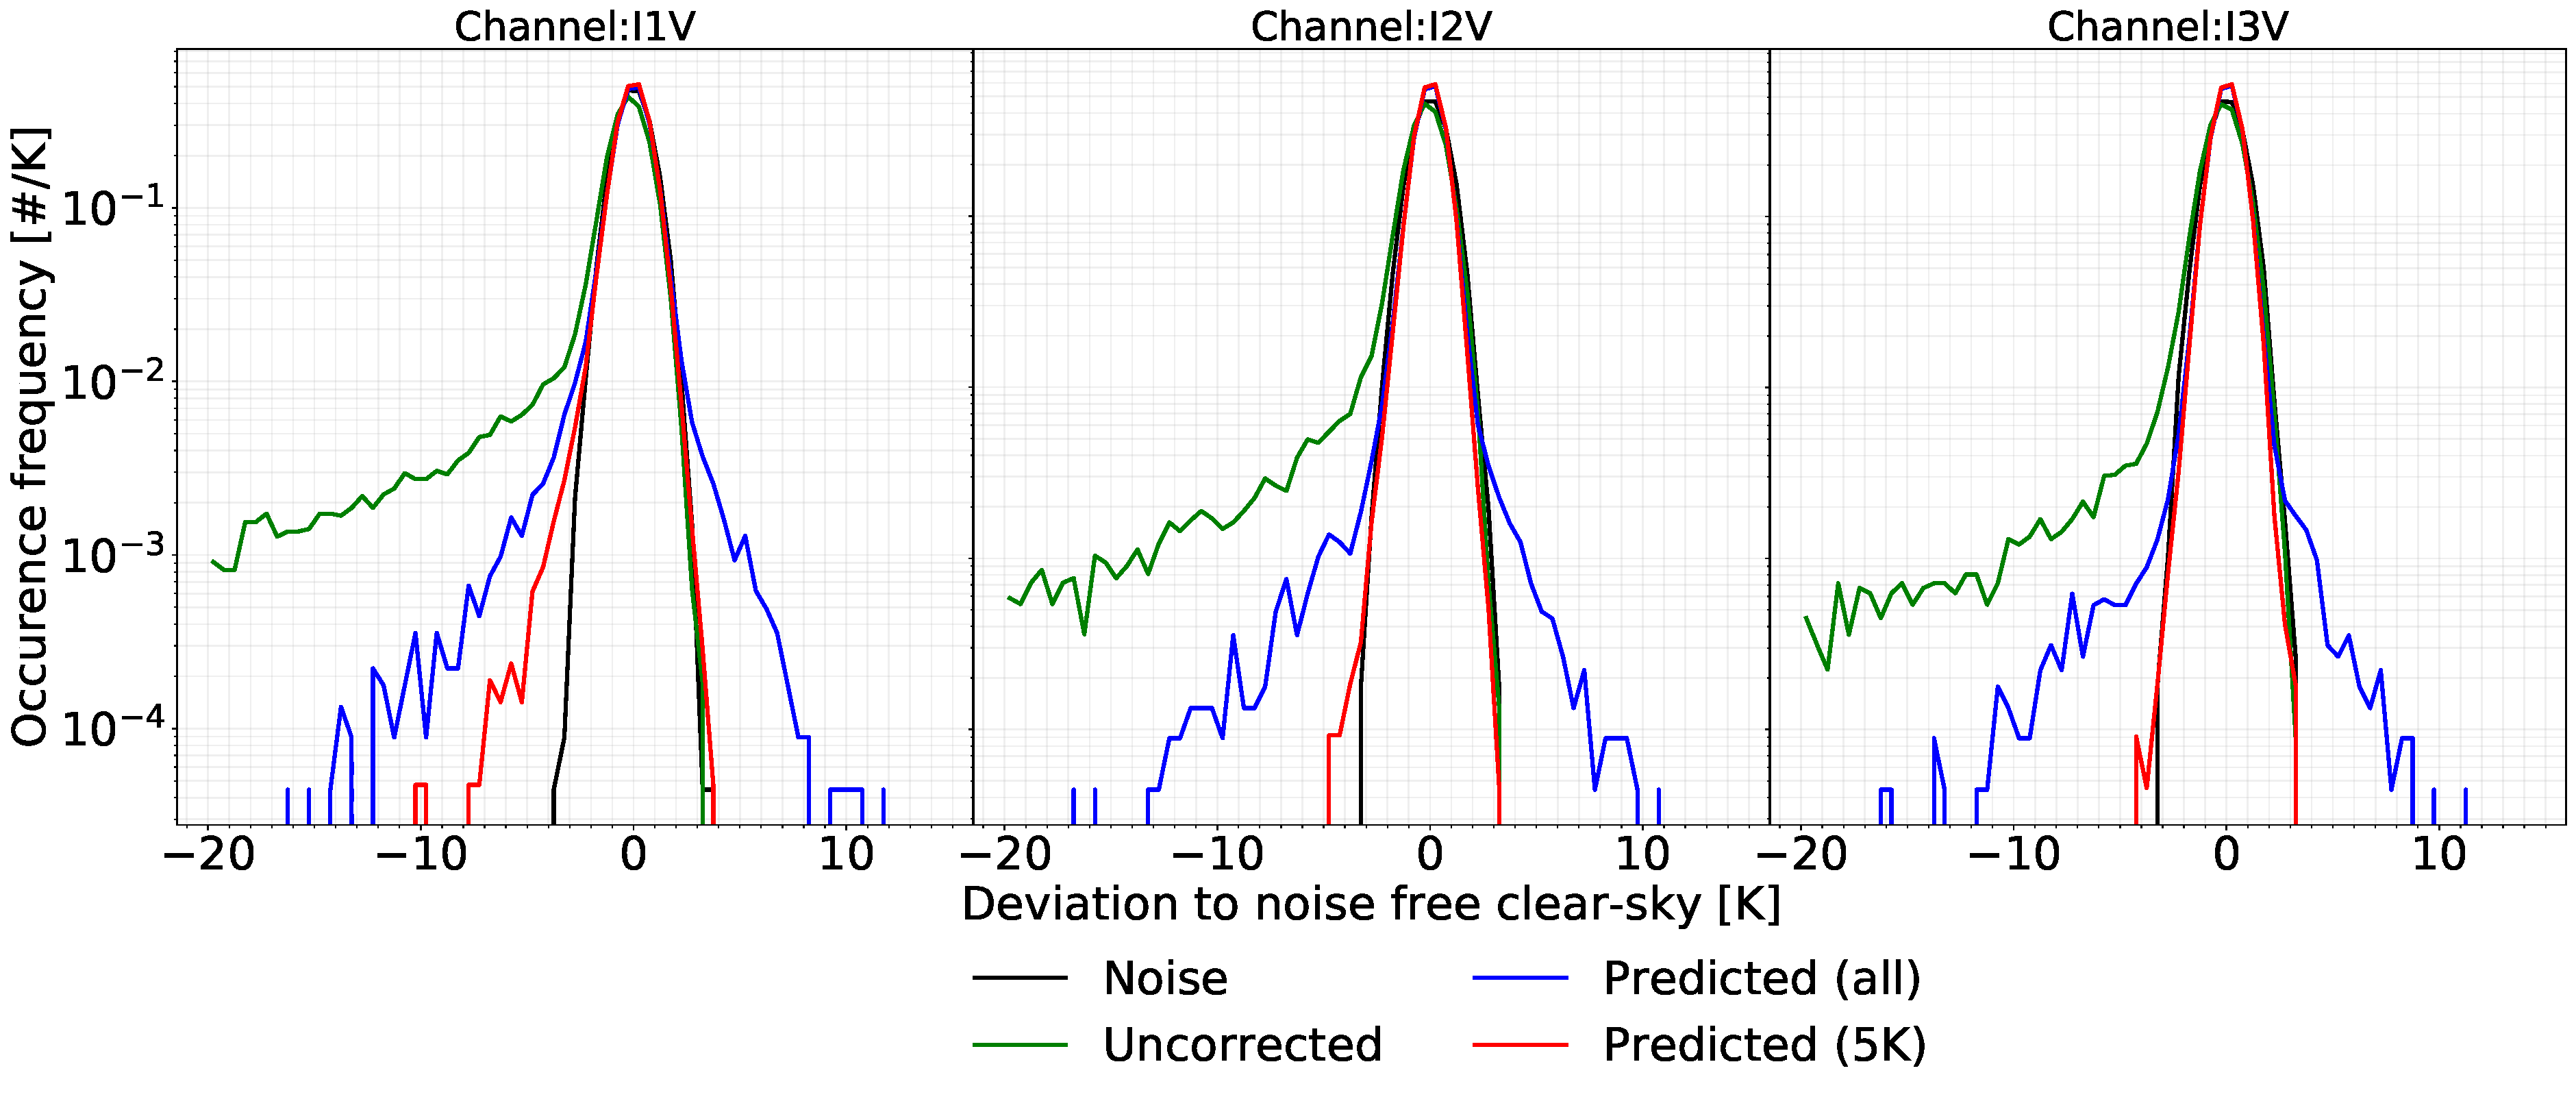
\includegraphics[width=\textwidth]{Figures/error_distribution_QRNN-single.pdf} 
	\caption{Error distributions for deviations of QRNN-simple predictions to clear-sky simulations for channels I1V, I2V and I3V. Label ``Uncorrected'' represents the measurements and ``Filtered(5\,K)'' represents the dataset when no correction is made but cases with cloud correction greater than 5\,K are omitted. `Predicted'' denotes the entire prediction dataset, while ``Predicted(5\,K)'' refers to the predicted dataset where cases with cloud correction greater than 5\,K are excluded.}
	\label{fig:error_distributions}	
\end{figure*}

%t
\begin{table*}[t]
	\caption{Bias, mean absolute error(MAE), standard deviation(STD), and measure of skewness(Skewness) for error distributions of predictions of I1V, I2V and I3V. Results from both QRNN-simple and QRNN-all are shown. The label ``Filtered'' refers to the dataset where cases with cloud correction greater than 5\,K are filtered out, and  no other correction is made. The label ``Predicted(All)'' refers to the complete predicted dataset, while in ``Predicted (5\,K)'', cases with cloud correction greater than 5\,K are removed from the predicted dataset. The fraction of cases removed by this filter are given in parentheses.}
	\label{tab:error_statistics_ici}
%	\tabcolsep=0.11cm
	\begin{tabular}{llrr|rrr|rrr}
		\tophline
		&&\multicolumn{2}{c|}{Simulations}& \multicolumn{3}{c|}{QRNN-single} & \multicolumn{3}{c}{QRNN-all}\\
		\cline{3-10}
%		\hline
		&&   Clear-sky &   All-sky &  Filtered & Predicted & Predicted &   Filtered & Predicted & Predicted \\
		&&&&							(5\,K) &(All)& (5\,K) & (5\,K)&(All)& (5\,K)\\
		\middlehline
%		\multicolumn{7}{c}{Channel - I1V}\\

Channel I1V& Bias     &  0.00 & -1.88 & -0.32(6.1\%) & -0.06 & -0.04 & -0.31(6.1\%) & -0.06 & -0.04 \\
			&MAE      &  0.64 &  2.32 &  0.79 &  0.64 &  0.55 &  0.78 &  0.61 &  0.54 \\
			&STD      &  0.80 &  8.84 &  1.07 &  0.98 &  0.73 &  1.07 &  0.91 &  0.71 \\
			&Skewness & -0.01 & -8.10 & -1.53 & -1.53 & -0.75 & -1.52 & -1.07 & -0.55 \\
\middlehline
Channel I2V &Bias     & -0.00 &  -1.04 & -0.24(3.7\%) & -0.01 & -0.00 & -0.24(3.6\%) & -0.05 & -0.03 \\
			&MAE      &  0.64 &   1.52 &  0.74 &  0.52 &  0.46 &  0.75 &  0.44 &  0.39 \\
			&STD      &  0.80 &   5.95 &  0.99 &  0.82 &  0.59 &  0.99 &  0.67 &  0.50 \\
			&Skewness &  0.00 & -10.80 & -1.10 & -2.17 & -0.27 & -1.05 & -2.22 & -0.27 \\
\middlehline	
Channel I3V &Bias     & -0.00 &  -0.63 & -0.18(2.3\%) &  0.01 &  0.02 & -0.19(2.2\%) & -0.03 & -0.03 \\
			&MAE      &  0.64 &   1.15 &  0.71 &  0.51 &  0.47 &  0.72 &  0.46 &  0.42 \\
			&STD      &  0.80 &   4.27 &  0.93 &  0.77 &  0.59 &  0.95 &  0.68 &  0.54 \\
			&skewness & -0.00 & -13.41 & -0.86 & -1.75 & -0.11 & -0.93 & -1.53 & -0.14 \\
		\bottomhline
	\end{tabular}
	\belowtable{} % Table Footnotes
\end{table*}

\begin{table*}[t]
	\caption{A comparison of the error statistics from QRNN-single and QRNN-all, when only cases with cloud correction greater than 10\,K are included. The fraction of cases forming the dataset are included in the parentheses}
	\label{tab:error_statistics_ici_high_cloud_impact}
	%	\tabcolsep=0.11cm
	\begin{tabular}{lrr|rr|rr}
		\tophline
		&\multicolumn{2}{c|}{I1V}& \multicolumn{2}{c|}{I2V} & \multicolumn{2}{c}{I3V}\\
		\cline{2-7}
		&QRNN-single& QRNN-all & QRNN-single & QRNN-all  & QRNN-single & QRNN-all\\
		\middlehline
				    Bias     & -0.53(4.02\%) & -0.38(4.07\%)  & -0.42(2.26\%) & -0.46(2.25\%) & -0.25(1.32\%) & -0.40(1.28\%) \\
					MAE      &  2.32 &  1.93  &  2.77 &  2.08 &  3.10 &  2.59 \\
					STD      &  3.13 &  2.63  &  3.65 &  2.85 &  4.03 &  3.47 \\
		\bottomhline
	\end{tabular}
	\belowtable{} % Table Footnotes
\end{table*}


\begin{figure}[t]
	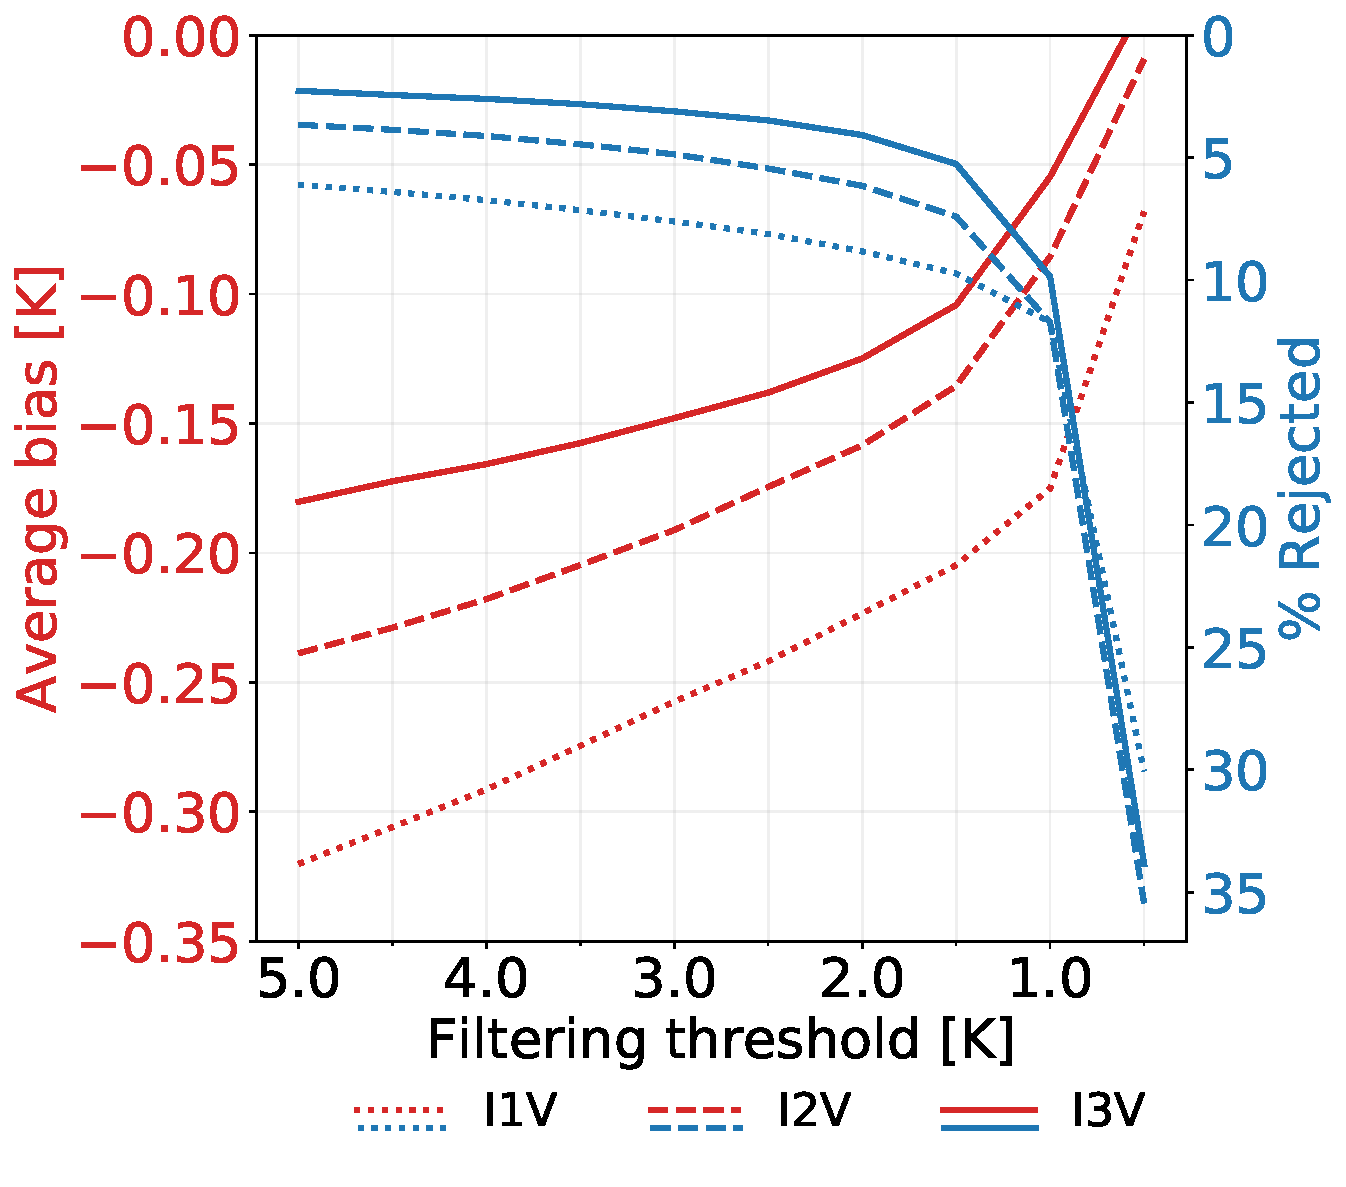
\includegraphics[width=70mm]{Figures/different_filtering_thresholds.pdf} 
	\caption{A comparison of the  average error bias when pure-filtering approach (QRNN-single) is applied with different thresholds (red curves). The corresponding fraction of cases rejected is also shown on the right y-axis(blue curves).}
	\label{fig:filtering_thresholds}	
\end{figure} 
To assess the accuracy of QRNN predictions, a point estimate of the posterior distribution is required. Usually for Bayesian analysis, the posterior mean or posterior median are selected as point estimates. In this study, we assume the posterior median to be the best estimate for the predicted clear-sky value. 

The distributions of median value of clear-sky predictions from QRNN-single are shown in Fig.~\ref{fig:PDF_predictions}. The distributions of corresponding NFCS simulations are also plotted as reference. The three figures correspond to channels: I1V, I2V and I3V. These results show that the clear-sky values predicted by QRNN-single have a very good match for the peak of the distributions, but a slight mismatch is evident towards the tails. The degree of mismatch is highest for I1V, which incidently also has the largest spread of brightness temperatures in the clear-sky conditions. For all three channels, the colder brightness temperatures are under-estimated by QRNN, while a tendency to over-estimate the warmer brightness temperatures is seen for I1V and I2V.  
  
For a quantitative evaluation of QRNN accuracy, the prediction errors are calculated as the deviation of the best estimate to its corresponding NFCS values. We calculate the mean bias, MAE (mean absolute error) and standard deviation of the errors. The asymmetry of error distributions around their mean is also calculated through the measure of skewness. Fisher-Pearson coefficient of skewness is used to calculate the measure of skewness: 
\begin{equation}
g_1 = \frac{m_3}{m_2^{3/2}}, 
\end{equation}
where $m_2$ and $m_3$ are biased sample's second and third central moments. 

Fig~\ref{fig:error_distributions} shows the error distributions of predictions for all three channels from QRNN-single. The distribution of noise is also plotted for reference. Without any cloud impact, the error distributions should follow a Gaussian distribution, and the skewness should be close to zero. However the presence of clouds leads to a brightness temperature reduction, and introduces a high negative bias among the deviations. Among the three channels, I1V has the highest cloud impact, while I3V has the least. After correction of the cloud impact, the resulting error distributions are  symmetric with a sharper peak albeit with a large spread. The large spread is due to cases which end up with partial cloud correction and also due to cases where the predicted values are warmer than the simulations. For all three channels quite similar behaviour is observed, though I1V has the highest number of cases with residual cloud impact. We assume that such cases are associated with high cloud impact. To validate our assumption, we implemented a pure-filtering approach. In the filtered subset, we removed all cases with QRNN cloud correction greater than 5\,K, and did not correct the remaining cases. This can be considered as a pure-filtering approach. The results from this subset are also displayed in the figure (red curve). For all three channels, the right side follows measurement noise, as expected, but the left side has substantial cases with small cloud impact which pass through the filter. However, since the spread of filtered dataset is smaller than the corrected one, it confirms our assumption that most of the partially corrected cases have high cloud impact. On the other hand, if all the predicted cases with correction less than 5\,K (Predicted (5\,K) in the figure) are considered, the resulting error distributions are quite close to the measurement noise, except for I1V, where few cases with residual cloud impact can still be seen. 

The error metrics corresponding to the error distributions described above are provided in Table~\ref{tab:error_statistics_ici}. The average bias in channel I1V measurements is -1.88\,K, which reduces to -0.32\,K with pure-filtering. However, when the complete dataset is corrected, the bias is only -0.06\,K and the standard deviation is only 0.98\,K in comparison to 8.84\,K in the measurements.  The prediction accuracy of QRNN is further higher when filtering is made on the corrected data. In this case, the residual bias is only -0.04\,K, and the standard deviation is 0.73\,K, which is in fact of the order of measurement noise (0.80\,K). This high accuracy is achieved by filtering just 6.1\% of the data. This indicates that though a pure-filtering approach can prove as a reliable procedure for removing cases with high cloud impact, it is important to correct cases with relatively low cloud impact. 

Similar results are seen for channel I2V, though a better performance of QRNN is observed. In I2V, the measurement bias is -1.04\,K which reduces to -0.01\,K after correction. The MAE also reduces from 1.52\,K to 0.52\,K. Removing cases with correction greater than 5\,K from the corrected dataset removes only 3.7\% of the data but reduces the absolute error to 0.46\,K and the bias to 0\,K. The standard deviation of the resulting dataset is only 0.59\,K as compared to 0.80\,K from noise. The reduction in the variability is also evident in the Fig~\ref{fig:error_distributions}, where the peak of the predicted distributions is sharper.

In comparison to I1V and I2V, I3V has the lowest fraction of the measurements with significant cloud impact. The bias in the measurements is only -0.63\,K in comparison to -1.88 in I1V. Pure-filtering removes 2.3\% of the total cases as cloudy, reduces the bias to 0.18\,K, and the standard deviation to 0.91\,K but nonetheless, cannot provide a complete cloud filtering. After correction of all the cases in the test dataset, the bias reduces to 0.01\,K and the MAE to 0.51\,K from 1.15\,K. Including correction along with filtering reduces the bias further down to 0.02\,K and standard deviation to 0.59\,K, which is again smaller than that of noise(0.80\,K).

Overall for all three channels, the accuracy of the predicted dataset with correction greater than 5\,K removed, gives the best accuracy and lowest variability. Although similar results can also be achieved by selecting a lower filtering threshold, it comes at the cost of rejecting higher fraction of cases. Fig~\ref{fig:filtering_thresholds} shows the average errors obtained from different filtering thresholds and the corresponding percentage of data omitted (blue curve) for all three channels. Lowering the filtering threshold from 5\,K to 2.5\,K has only a small effect on improving the accuracy, however with further lower threshold values, accuracy of the order of ``predicted(5\,K)'' can be achieved, nonetheless with a high rejection. For example, for I1V, when all cases with cloud correction greater 0.5\,K are filtered, the average error bias of the subset is -0.06\,K, the MAE is 0.59\,K and the standard deviation is 0.75\,K. Though, these values are comparable to predicted cases with 5\,K filter, they come at the cost of rejecting more than 30\% of the total cases. The unusually high rejection rate indicates that using lower filtering thresholds elevates the risk of erroneously removing clear-sky cases.  

Next, we describe the results from QRNN-all. In this model, all 183\,GHz channels along with other sub-mm channels were included while training. This model was designed to identify if other channels of the same frequency can provide auxiliary information in the training process. The results from QRNN-all all are also provided in the last columns of Table~\ref{tab:error_statistics_ici}. For channel I1V, using additional information from other two 183\,GHz channels has no impact on pure-filtering approach but a slight positive impact on the predictions. If predictions over the entire testing set are considered, the average bias in QRNN-all and QRNN-single is same, but the mean absolute errors in QRNN-all are almost 4.5\% less than QRNN-single, suggesting a lower spread of errors. Having said that, in comparison to QRNN-single, the prediction accuracy has no significant improvement when all cases with correction larger than 5\,K are rejected. Thus, information from other 183\,GHz channels only assists in slightly improving the correctness of cases associated with high cloud impact in I1V. The accuracy of other cases remains unaltered. In order to quantify the positive effect on cases with high cloud impact, we computed the error statistics for all cases with correction greater than 15\,K. The results are shown in Table~\ref{tab:error_statistics_ici_high_cloud_impact}. For I1V, only 4\% of the cases have cloud correction greater than 10\,K, but have lowest prediction accuracy. Using QRNN-all improves the overall error bias from -0.53\,K to -0.38\,K and the standard deviation from 3.13\% to 2.63\%,but still is unsuccessful in removing the cloud impact completely. Lower representation of cases with high cloud impact in the training set could be one of the reasons for this shortcoming. Due to low fraction of such cases, QRNN cannot learn to predict the clear-sky values accurately.  

For channel I2V, the predictions from QRNN-all have a slightly worse average error bias than QRNN-single, yet a significant improvement in the prediction accuracy is evident. For the complete testing set, the MAE is 0.44\,K in comparison to 0.52\,K from QRNN-single, showing an improvement of almost 15\%. Similarly the standard deviation of the errors is only 0.67\,K, notably smaller than the measurement noise. Additionally, when the  corrected dataset is filtered with 5\,K threshold, the accuracy is even better. The mean absolute bias reduces to 0.39\,K and standard deviation to 0.50\,K. This implies that cases pertaining to clear-sky conditions and relatively low cloud impact benefit the most from the auxiliary information. This is in contrast to channel I1V, where accuracy of such cases remained unaffected. However, for cases with cloud impact greater than 10\,K a likewise improvement is observed (Table~\ref{tab:error_statistics_ici_high_cloud_impact}). Again both QRNN-all and QRNN-single are only partially successful in removing the cloud impact, but QRNN-all had a better performance among the two. For I2V, such cases form only 2.25\% of the testing dataset. Predictions from QRNN-all have slightly worse values for average error bias, but both MAE and standard deviation improve by over 20\%.
   
For channel I3V, the performance of QRNN-all is comparable to that for I2V. For I3V, the mean absolute bias in QRNN-all is 0.46\,K compared to 0.51\,K from QRNN-single, and the corresponding standard deviations are 0.68\,K and 0.77\,K. Removing the cases with cloud impact greater than 5\,K from the predicted dataset, leads to no change in the average bias, but the mean absolute error and standard deviation reduce by almost  8\% and 20\% respectively. Again suggesting that cases with low/no cloud impact have a significant contribution in improving the accuracy of predictions. Cases with high cloud impact, though very low in number, also gained positively from the auxiliary information.  

\subsubsection{Uncertainty quantification}
\label{sec:prediction_uncertainty}
%f 
\begin{figure}[t]
	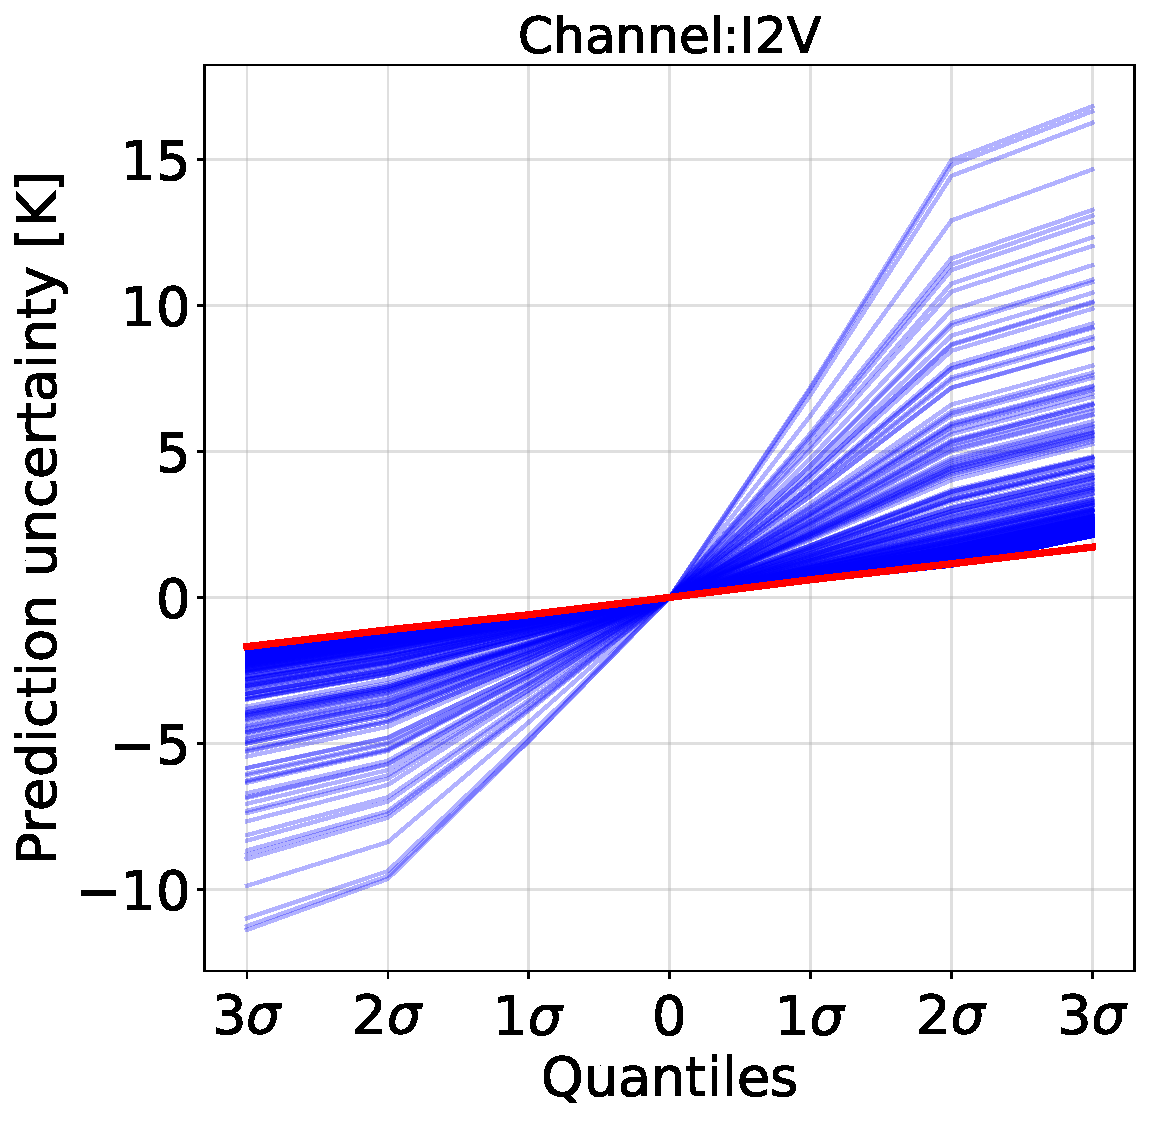
\includegraphics[width = 70mm]{Figures/prediction_uncertainty_I2V.pdf}	
	\caption{The prediction uncertainty  for I2V  with respect to quantiles for randomly selected 1500 cases. The black line represents the uncertainty if underlying distribution is purely Gaussian with mean 270\,K and standard deviation 0.60\,K. The results are from QRNN-single.}
	\label{fig:prediction_uncertainty_I2V}	
\end{figure}
\begin{figure}[t]
	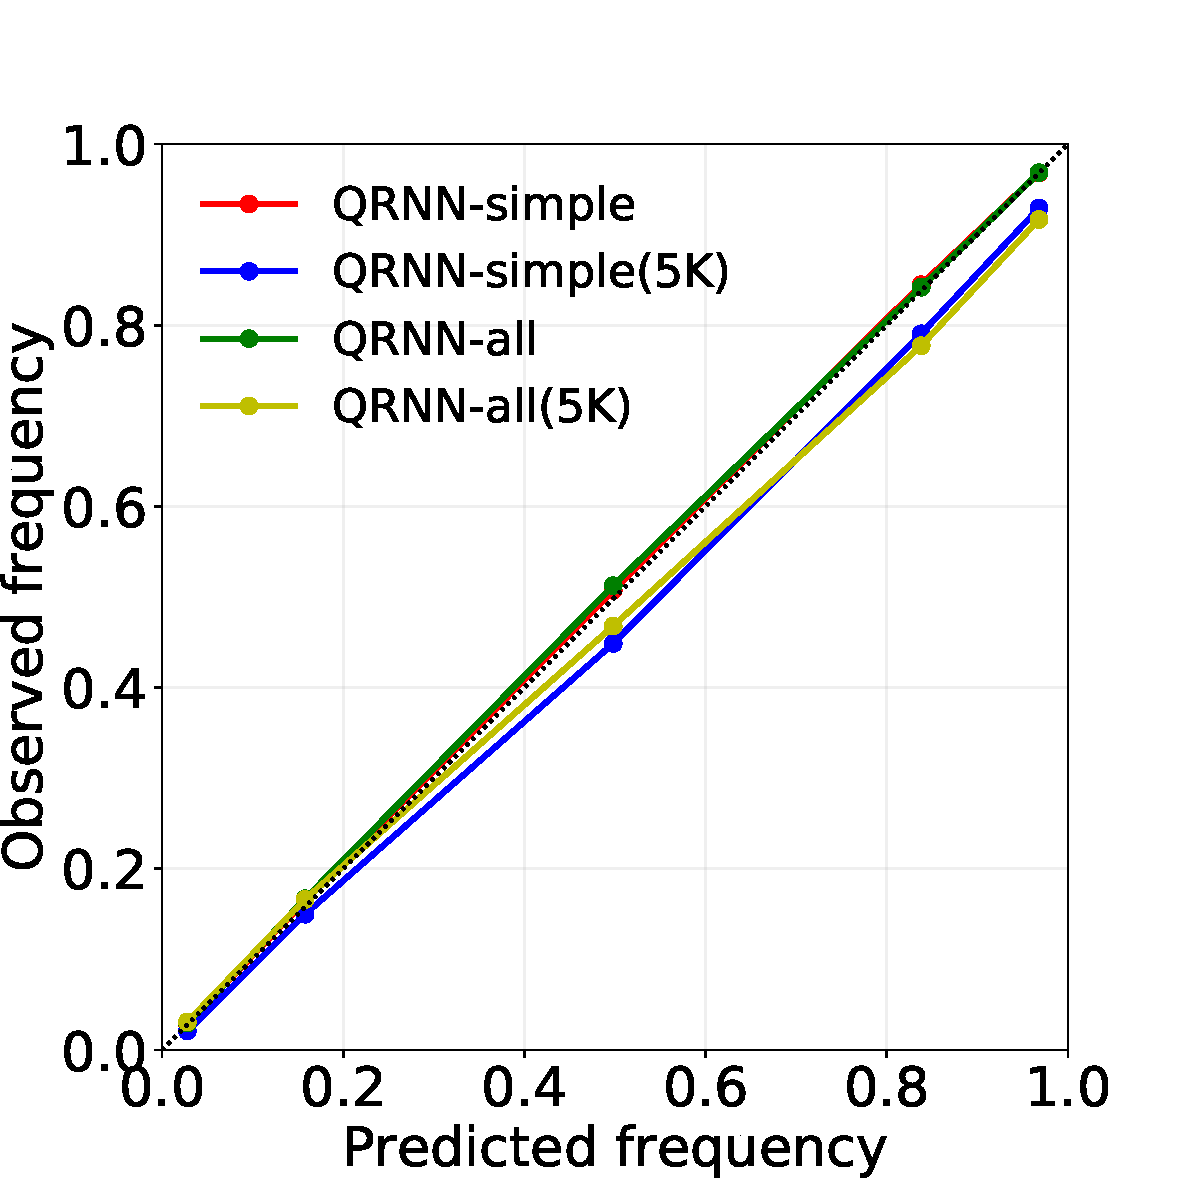
\includegraphics[height = 70mm]{Figures/calibration_QRNN_I1V.pdf}	
	\caption{Calibration of the prediction intervals obtained from QRNN-simple and QRNN-all for channel I1V. }
	\label{fig:calibration_I1V}	
\end{figure}
\begin{figure*}[t]
	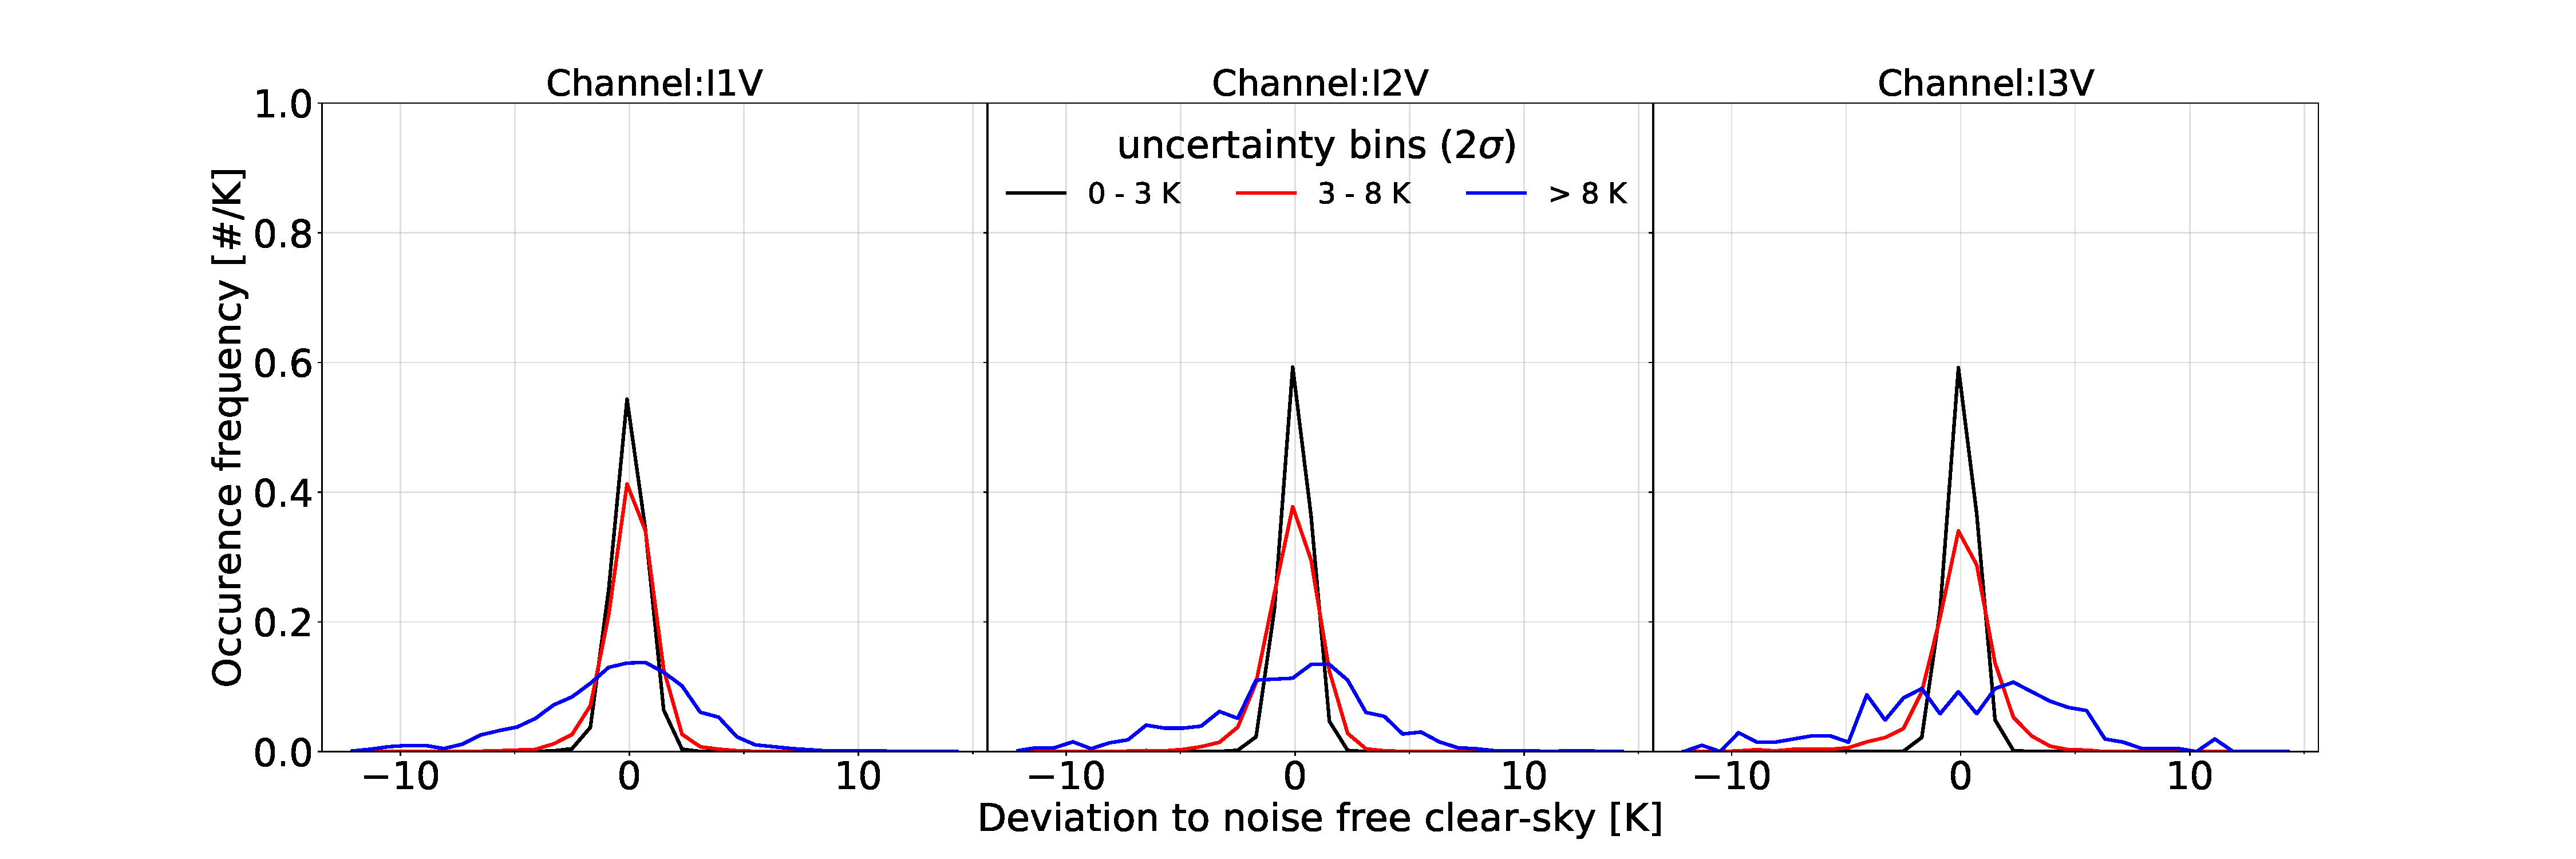
\includegraphics[width=\textwidth]{Figures/PDF_uncertainty_bins_QRNN-single.pdf}	
	\caption{Distribution of errors binned according to their uncertainty. Results are from QRNN-single for channels I1V, I2V and I3V.}
	\label{fig:error_distribution_uncertainty_bins}	
\end{figure*}

The biggest advantage of using QRNN is estimation of case-specific uncertainties. The quantiles can be used to construct a probability distribution of the predictions in contrast to other correction approaches which give out only point estimates. If median is chosen as the point estimate, the predictions at other quantiles provide a measure of the possible fluctuations in the point estimate. 

In order to understand how QRNN predicted uncertainties behave, we calculated the deviations of predictions at different quantiles from the median value. Fig.~\ref{fig:prediction_uncertainty_I2V} displays the prediction uncertainty in I2V for different quantiles. The different lines represent 1500 randomly chosen cases, while the black line represents the uncertainty in a hypothetical Gaussian distribution of $270\pm0.60$\,K, which is of the order of standard deviation for I2V predictions (see Table~\ref{tab:error_statistics_ici}). The uncertainty estimates from different cases show a very high degree of variability. Among the cases associated with low uncertainty, the distribution is quite symmetric along the median value. Such cases are concentrated along a narrow interval and lie close to the black curve. For such cases, the uncertainties are also equally spaced for $1\sigma$, $2\sigma$ and so on, suggesting that a Gaussian distribution model could be used to express the underlying uncertainty of such cases. However, cases with high uncertainty have a larger spread, and are no longer equally spaced. For these cases, the prediction uncertainties have a larger spread over positive quantiles than negative quantiles.  The high variability indicates that QRNN can successfully represent uncertainties for each case individually, rather than expressing them as a single measure for all cases. In the latter case, the uncertainty estimates for all cases would be concentrated along a narrow interval. 

For further analysis of the uncertainty estimates, we compare the distributions of the predictions from QRNN with the a priori distribution. In a model with high performance, the posterior distribution of the predictions should be similar to the a priori distribution of training dataset. A straightforward way to compare the two distribution is to plot the frequency of predictions and frequency of true value in different prediction intervals. This is also commonly known as calibration plot. Fig.~\ref{fig:calibration_I1V} shows the calibration of the prediction intervals on the test dataset for channel I1V. Results from both QRNN-single and QRNN-all are shown. The calibration of predictions with correction greater than 10\,K is also shown. For both QRNN models, the predictions for the complete test dataset are well calibrated and follow the y=x line. This shows that the training and test datasets come from the same a priori distribution. On the other hand, when cases with  cloud correction greater than 10\,K are considered, for both models, the predictions in all the intervals are poorly calibrated. In this case the calibration curve lies below the y=x line, indicating that the predicted intervals are too narrow, or the uncertainty is underestimated.  In the test and training datasets, the clear-sky cases and cases with low cloud impact dominate the a priori distribution, and cases with high cloud impact fail to get an adequate representation. The a priori distribution of such cases is different from the clear-sky cases, thus the corresponding predictions had poor calibrations.  We also plotted the calibration curves for I2V and I3V (figure not shown). For both these channels, predictions over complete dataset were well calibrated for both QRNN-single and QRNN-all, but for subset with threshold 10\,K, the slightly poor calibrations were observed in QRNN-single. This is in contrast with I1V, where both models had poor calibrations for cases with high cloud impact. 

Lastly, we investigated that if the uncertainty estimates given by QRNN are representative of prediction errors.  We divided the 94\% confidence interval ($\pm2\sigma$ ) into three bins and estimated the prediction error distribution for each.  Fig.~\ref{fig:error_distribution_uncertainty_bins} shows the prediction error distributions for I1V, I2V and I3V. These results are from QRNN-single. Similar results were also obtained for QRNN-all (figure not shown). For all three channels, an increase in the prediction errors with uncertainty is observed. The cases with high certainty have a narrow and sharp distribution, and the errors are mostly less than $\pm$2.5\,K. With increase in the uncertainty, frequency of cases with high accuracy decreases and the distributions spread out symmetrically to higher errors. Poor predictions occur more frequently when uncertainty is high, although cases with accurate predictions yet high uncertainty are also present. In spite of individual variations in the error distributions of each channel, predictions and their corresponding uncertainties followed the same relationship: This suggests that QRNN can reliably represent the quality of predictions through their uncertainty estimates.

These three different types of analysis show that both QRNN-single and QRNN-all are successful in providing well calibrated probabilistic predictions of the posterior distributions except for few cases associated with high cloud impact. This is not unexpected, as such cases form a small subset of the training set and their priori distribution could be different from the entire dataset. Since such cases form only a fraction of the training dataset, it can be hard to train the model to predict them accurately. A larger training dataset would be required to increase the representation of such cases in QRNN.


\subsection{MWI}
%
In this section, we present results from QRNN when applied to MWI channels. Applicability and sensitivity of QRNN over different combinations of training datasets, is investigated. Firstly, we use combinations of data from all five 183\,GHz channels for ``self'' cloud filtering/correction (QRNN-mwi). No additional data is used. In the second model, we compare the performance of QRNN for MWI channels, if sub-mm channels from ICI are used. In this case, we assume that data from both channels is mapped to a common foorprint size.
\subsubsection{MWI alone}
%
%t
\begin{table*}[t]
	\caption{Error statistics for predictions from QRNN-mwi. All channels of MWI are used to train for each 183\,GHz channel. The labels Filtered(5\,K), Predicted(All) and Predicted(5\,K) are same as described in Table~\ref{tab:error_statistics_ici}}
	\label{tab:statistics_mwi-alone}
	\begin{tabular}{llrr|rrr}
		\tophline
		&&\multicolumn{2}{c|}{Simulations}& \multicolumn{3}{c}{QRNN-single} \\
		\cline{3-7}
		%		\hline
		&&   Clear-sky &   All-sky &  Filtered(5\,K) & Predicted & Predicted(5\,K) \\
		\middlehline
		MWI-14 		&bias     & 0.00 & -1.87 & -0.45 & -0.18 & -0.15 \\
					&mae      & 0.64 &  2.31 &  0.91 &  0.96 &  0.80 \\
					&std      & 0.81 &  8.97 &  1.54 &  1.73 &  1.29 \\
					&skewness & 0.03 & -8.32 & -4.02 & -1.09 & -3.06 \\
		\middlehline
		MWI-15 		&Bias     & -0.01 & -1.23 & -0.36 & -0.16 & -0.13 \\
					&MAE      &  0.64 &  1.70 &  0.85 &  0.62 &  0.53 \\
					&STD      &  0.80 &  6.48 &  1.33 &  1.23 &  0.97 \\
					&skewness &  0.01 & -9.96 & -3.32 & -3.06 & -4.17 \\
		\middlehline	
		MWI-16 		&Bias     & -0.00 &  -0.84 & -0.26 & -0.15 & -0.12 \\
					&MAE      &  0.64 &   1.35 &  0.78 &  0.53 &  0.47 \\
					&STD      &  0.80 &   5.31 &  1.15 &  1.03 &  0.80 \\
					&skewness & -0.01 & -12.08 & -3.05 & -5.09 & -4.94 \\	
		\middlehline			
		MWI-17 		&Bias     & -0.00 &  -1.06 & -0.31 & -0.16 & -0.12 \\
					&mae      &  0.64 &   1.54 &  0.80 &  0.62 &  0.54 \\
					&std      &  0.80 &   6.22 &  1.22 &  1.12 &  0.90 \\
					&skewness &  0.01 & -11.06 & -3.31 & -4.35 & -4.33 \\	
		\middlehline			
		MWI-18 		&Bias     & -0.00 &  -0.66 & -0.23 & -0.11 & -0.08 \\
					&mae      &  0.64 &   1.17 &  0.76 &  0.62 &  0.57 \\
					&std      &  0.80 &   4.57 &  1.13 &  1.08 &  0.88 \\
					&skewness &  0.01 & -13.56 & -3.28 & -4.67 & -3.80 \\	
		\bottomhline				
	\end{tabular}	
	\belowtable{} % Table Footnotes
\end{table*}
QRNN-mwi is designed to provide basis for a cloud correction approach applicable to current satellites, which lack the higher frequency channels. Table~\ref{tab:statistics_mwi-alone} shows the results for all 183\,GHz channels of MWI. For MWI-14, the predictions from QRNN-mwi are only partially successful in removing the cloudy impact. The prediction errors for the complete testing dataset are highly symmetric but with a large spread. The average error bias of measurements from NFCS values is -1.87\,K, and after correction, it reduces to -0.18\,K. The corresponding standard deviation values are 9.01\,K and 1.87\,K. When cases with 5\,K correction are filtered out from the predicted dataset, the bias reduced further to -0.16\,K and MAE from 1.13\,K to 0.97\,K. Though there is a small increase in the accuracy, the high errors indicate residual cloud impact. For MWI-15, a slightly better accuracy than MWI-14 is observed. For this channel, the average error bias in the measurements is -1.23\,K, which  reduces -0.15 after correction.  
\subsubsection{MWI and ICI}
%t
\begin{table*}[t]
	\caption{Same as Table~\ref{tab:error_statistics_ici}, but for channels MWI-15 and MWI-16. Results are from QRNN-single.}
	\label{tab:statistics_mwi}
	\begin{tabular}{llrr|rrr}
		\tophline
				&&\multicolumn{2}{c|}{Simulations}& \multicolumn{3}{c}{QRNN-single} \\
				\cline{3-7}
				%		\hline
				&&   Clear-sky &   All-sky &  Filtered(5\,K) & Predicted & Predicted(5\,K) \\
		\middlehline
		MWI-15  &Bias     &  0.00 & -1.23 & -0.26 & -0.04 & -0.03 \\
				&MAE      &  0.64 &  1.70 &  0.76 &  0.56 &  0.50 \\
				&STD      &  0.81 &  6.48 &  1.01 &  0.86 &  0.64 \\
				&Skewness & -0.00 & -9.97 & -1.15 & -1.78 & -0.15 \\
		\middlehline
		MWI-16  &Bias     & 0.00 &  -0.85 & -0.22 & -0.06 & -0.05 \\
				&MAE      & 0.64 &   1.34 &  0.73 &  0.55 &  0.50 \\
				&STD      & 0.80 &   5.31 &  0.96 &  0.83 &  0.63 \\
				&Skewness & 0.01 & -12.08 & -1.02 & -2.25 & -0.11 \\
		\bottomhline			
	\end{tabular}	
	\belowtable{} % Table Footnotes
\end{table*}
In this section, we combine the measurements from MWI-15(MWI-16) and the ICI sub-mm channels to predict MWI-15(MWI-16). Since we assume that all channels are remapped to a common footprint, channels MWI-14, MWI-17 and MWI-18 are virtually identical to I1V, I2V and I3V, and thus results for them are not shown separately. Table~\ref{tab:statistics_mwi} shows the metrics from error distributions for MWI-15 and MWI-16 predictions. Results from only QRNN-single are shown. 

For MWI-15, the average deviations of measurements from NFCS values is -1.23\,K, and the MAE is 1.70\,K. When all cases are corrected, the resulting average bias is -0.04\,K and the MAE reduces to 0.56\,K. If only pure-filtering is made, the average bias is -0.26\,K and MAE is 0.76\,K, suggesting that a significant number of cases non-zero cloud impact pass through. As seen for ICI, best results are obtained  when filtering is made on the corrected dataset. 
Similar accuracy is seen for MWI-16, although it has slightly lower cloud impact.




\subsection{AWS}
In this section, we investigate the possibility of using only channels around 325\,GHz for cloud correction at 183\,GHz. This special case of utilising only 325\,GHz channel can be relevant for smaller satellite missions like Artic Weather Satellite (AWS) where higher sub-mm channels are not available. 

In an analogy between the results from ICI channels, we perform a similar error distribution analysis 
and the results are displayed in Table~\ref{tab:statistics_qrnn_aws}. For channel AWS-32, the average bias and standard deviation in the prediction errors is is -1.34\,K and 5.91\,K respectively. However, after correction, the bias and standard deviation are -0.08\,K and 1.0\,K. A decrease in the skewness of error distributions is evident(from -7.48 to -1.52), but a relatively high values after prediction indicate presence of cases with partially-corrected cloud impact. For AWS-33, the predictions have slightly higher accuracy than AWS-32. The MAE in predictions is only 0.50\,K in comparison to 1.23\,K for the measurements. Similar results are also seen for AWS-35 and AWS-36. For both channels, the predictions are relatively more symmetric than the other channels. Also, it is worth to noting that when cases with 5\,K cloud correction are removed, the spread of predictions is narrower than noise. 

Overall the results demonstrate that QRNN is successful in predicting the clear-sky noise-free data for AWS-33, AWS-34, AWS-35 and AWS-36 and partially for AWS-32. The prediction error distributions are symmetric with low bias and standard deviation. The cases with high error are mostly associated with high cloud impact and constitute only a small fraction of the total dataset. Excluding such cases decreases the variability in the predictions and in fact the spread of errors for AWS-34, AWS-35 and AWS-36 is smaller than noise. Removal of cases with high cloud impact, increases the representation of cases in cloud-free conditions, and for such cases, QRNN predictions can be seen as a weighted mean between the two ``super-channels''. Since the noise in the two channels are stationary and uncorrelated, the predictions benefit from the additional information, but the noise component tends to cancel out. For AWS-32, QRNN is only partially successful in reducing the impact of hydrometeors. The prediction errors have significantly lower spread than the measurements, but cases with partially corrected cloud impact deteriorates the overall accuracy. Since 325\,GHz cannot provide a full coverage for hydrometeor impact in AWS-32, the testing data will inevitably contain cases for which QRNN has not trained for. Prediction for such \textit{out-of-distribution} cases would be inaccurate and highly uncertain. In such cases, the predictions should be used with caution. 

In order to analyse the performance of QRNN with task difficulty, the interrelation between the uncertainty estimates and cloud impact was investigated. Here we assume that cloud impact is representative of task difficulty. Fig~\ref{fig:uncertainty_cloud_impact} displays the plot between mean uncertainty estimates for $2\sigma$ confidence interval and the cloud impact. For all five channels, the predictions with small or relatively low cloud signal have a low uncertainty or in other words have high sharpness. As fraction of cloud impact increases, the predictions become increasingly uncertain. However, this does not imply that the prediction accuracy is low. 

\begin{table*}[t]
	\caption{Bias, mean absolute error(MAE), standard deviation(STD), and measure of skewness(Skewness) for error distributions of predictions AWS channels. Results are from QRNN-single. The label ``All'' refers to the complete dataset, while in ``Filtered'', cases with cases with cloud correction greater than 5\,K(15\,K) are excluded from statistics. The fraction of cases removed by this filter are given in parentheses.}
	\label{tab:statistics_qrnn_aws}
	\begin{tabular}{llrr|rrr}
		\tophline
		&&\multicolumn{2}{c|}{Simulations}& \multicolumn{3}{c}{QRNN-single} \\
		\cline{3-7}
		%		\hline
		&&   Clear-sky &   All-sky &   		 All &   Filtered(5K)& Filtered(15K) \\
		\middlehline
AWS-32    &Bias     &   -0.00 &         -1.34 &           -0.08 &       		-0.07(5.30\%) & -0.08(2.50\%) \\
          &MAE      &    0.36 &          1.58 &            0.62 &        		 0.53 		  &	0.57	\\
          &STD      &    0.45 &          5.91 &            1.00 &        		 0.74 		  & 0.85\\
          &Skewness &    0.02 &         -7.48 &           -1.52 &       		-1.63 		  & -2.01\\
		\middlehline
AWS-33	  &Bias     &   -0.00 &         -0.98 &            0.01 &                 0.00(4.08\%)& 0.00(1.75\%)\\
		  &MAE      &    0.36 &          1.23 &            0.50 &                 0.43 	      & 0.46\\
		  &STD      &    0.45 &          4.70 &            0.77 &                 0.57 	      & 0.64\\
		  &Skewness &    0.01 &         -8.76 &           -0.40 &                -0.90  	  & -1.00\\

		\middlehline
AWS-34	  &Bias    &    0.00 &         -0.68 &            0.02 &                0.01(3.02\%)& 0.01(1.11\%) \\
		  &MAE      &    0.50 &          1.08 &            0.53 &                 0.47 		 & 0.50\\
		  &STD      &    0.63 &          3.69 &            0.78 &                 0.62 		 & 0.70\\
		  &Skewness &    0.02 &        -10.30 &           -0.34 &                -0.49 		 &-0.76	\\
		 \middlehline
AWS-35	 & Bias     &    0.00 &         -0.42 &            0.01 &                 0.01(1.92\%) & 0.01(0.70\%) \\
		 &MAE       &    0.50 &          0.83 &            0.50 &                 0.47 		   & 0.49\\
		 &STD       &    0.63 &          2.65 &            0.71 &                 0.60         & 0.65\\
		 &Skewness  &    0.01 &        -12.45 &           -0.15 &                -0.15         &-0.26\\
		 \middlehline
AWS-36   &Bias     &    0.00 &         -0.27 &            0.02 &                 0.02(1.30\%) & 0.02(0.31\%)\\
		 &MAE      &    0.70 &          0.90 &            0.67 &                 0.64 		  & 0.06\\
		 &STD      &    0.88 &          2.06 &            0.91 &                 0.81 		  &0.85\\
		 &Skewness &   -0.01 &        -12.00 &           -0.51 &                -0.15 		  &-0.12\\	 
		\bottomhline				
	\end{tabular}
	\belowtable{} % Table Footnotes
\end{table*}
%f
\begin{figure}[t]
	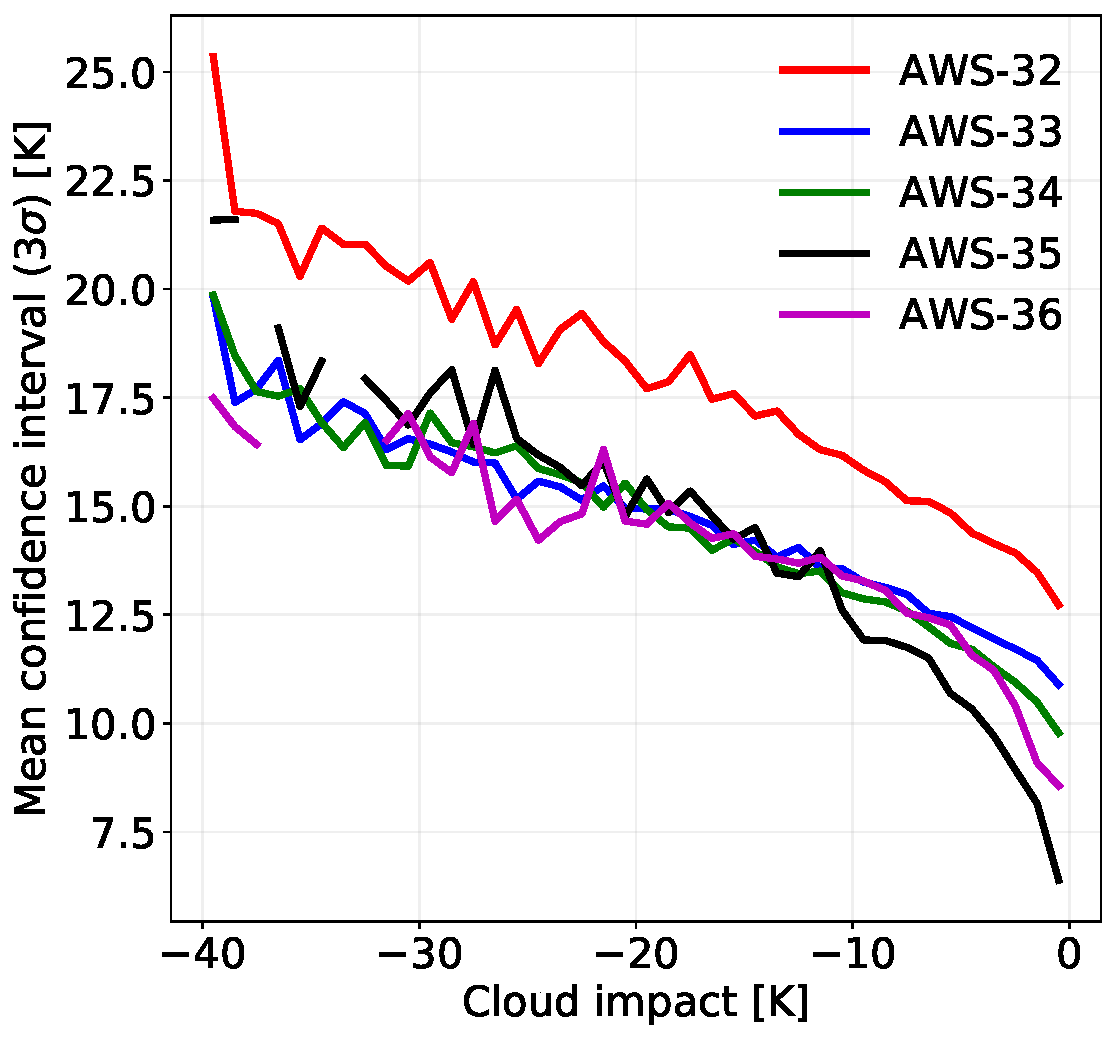
\includegraphics[width = 80mm]{Figures/cloud_impact_uncertainty_AWS.pdf}	
	\caption{The average confidence intervals (2$\sigma$) plotted against the magnitude of cloud impact for all AWS channels.}
	\label{fig:uncertainty_cloud_impact}	
\end{figure}
\section{Discussion}
\section{Outlook and Conclusions}  %% \conclusions[modified heading if necessary]


%% The following commands are for the statements about the availability of data sets and/or software code corresponding to the manuscript.
%% It is strongly recommended to make use of these sections in case data sets and/or software code have been part of your research the article is based on.

\codeavailability{TEXT} %% use this section when having only software code available


\dataavailability{TEXT} %% use this section when having only data sets available


\codedataavailability{TEXT} %% use this section when having data sets and software code available


\sampleavailability{TEXT} %% use this section when having geoscientific samples available


\videosupplement{TEXT} %% use this section when having video supplements available


\appendix
\section{}    %% Appendix A

\subsection{}     %% Appendix A1, A2, etc.


\noappendix       %% use this to mark the end of the appendix section. Otherwise the figures might be numbered incorrectly (e.g. 10 instead of 1).

%% Regarding figures and tables in appendices, the following two options are possible depending on your general handling of figures and tables in the manuscript environment:

%% Option 1: If you sorted all figures and tables into the sections of the text, please also sort the appendix figures and appendix tables into the respective appendix sections.
%% They will be correctly named automatically.

%% Option 2: If you put all figures after the reference list, please insert appendix tables and figures after the normal tables and figures.
%% To rename them correctly to A1, A2, etc., please add the following commands in front of them:

\appendixfigures  %% needs to be added in front of appendix figures

\appendixtables   %% needs to be added in front of appendix tables

%% Please add \clearpage between each table and/or figure. Further guidelines on figures and tables can be found below.



\authorcontribution{TEXT} %% this section is mandatory

\competinginterests{TEXT} %% this section is mandatory even if you declare that no competing interests are present

\disclaimer{TEXT} %% optional section

\begin{acknowledgements}
TEXT
\end{acknowledgements}




%% REFERENCES


 \bibliographystyle{copernicus}
 \bibliography{references.bib}

\end{document}
